\documentclass[twoside, 12pt]{epstfg}

\usepackage{lipsum}
\usepackage[numbers]{natbib}
%\usepackage{fancysprefs}
\usepackage{booktabs}
\usepackage{wrapfig}
\usepackage{enumitem}
\usepackage{xfrac}
\usepackage{multirow}
\usepackage{tikz}


\usetikzlibrary{arrows}
\usetikzlibrary{shapes}
\usetikzlibrary{patterns}
\usetikzlibrary{intersections}
\usetikzlibrary{calc}
\usetikzlibrary{fadings}

\definecolor{palette1}{HTML}{61d4b3}
\definecolor{palette2}{HTML}{fdd365}
\definecolor{palette3}{HTML}{fb8d62}
\definecolor{palette4}{HTML}{fd2eb3}
\definecolor{palette5}{HTML}{a7e9af}



\tikzstyle{IpNode}=[rectangle, draw=black, thick, inner sep=12pt]
\tikzstyle{NewIpNode}=[IpNode, fill=green]
\tikzstyle{MacNode}=[circle, draw=black, thick, inner sep=7pt]
\tikzstyle{NewMacNode}=[MacNode, fill=green]

\tikzstyle{OpenEdge}=[->, ultra thick]
\tikzstyle{CloseEdge}=[OpenEdge, red]
\tikzstyle{VirtualEdge}=[CloseEdge, double]
\tikzstyle{NewOpenEdge}=[OpenEdge, densely dashed]
\tikzstyle{NewCloseEdge}=[CloseEdge, densely dashed]
\tikzstyle{NewVirtualEdge}=[VirtualEdge, densely dashed]

\tikzset{>=latex}

\bibliographystyle{abbrv}

\title[spa]{Reconstrucción de caminos y detección de dispositivos}
\title[eng]{Path reconstruction and device detection}
\author{David Moreno Maldonado}
\tutor{Guillermo Julián Moreno}
\date[spa]{Junio 2020}
\date[eng]{June 2020}

\group[spa]{Naudit}
\group[eng]{Naudit}
\department[spa]{Ingeniería Informática}
\department[eng]{Information Technology}

\setdegreeDouble

%Resumen
%Abstract (resumen en ingles)

%Glosario
\newglossaryentry{ip}{
	name = {IP},
	description = {\textit{Internet Protocol}. En general, usado para referirse a una dirección IP}
}

\newglossaryentry{ttl}{
	name = {TTL},
	description = {\textit{Time To Live}. Contador del protocolo IP que decrementa al pasar de un nodo a otro}
}

\newglossaryentry{router}{
	name = {\textit{Router}},
	description = {Enrutador. Dispositivo que permite conectar hosts en una red. Se encarga de establecer la ruta de cada paquete dentro de dicha red}
}

\newglossaryentry{mac}{
	name = {MAC},
	description = {\textit{Media Access Control}. En general, usado para referirse a una dirección MAC que se corresponde de forma única con una tarjeta o dispositivo de red}
}

\newglossaryentry{pcap}{
	name = {Pcap},
	description = {Interfaz de una aplicación de programación para captura de paquetes. Su implementación para sistemas Unix es libpcap y el port para Windows es WinPcap}
}

\newglossaryentry{nat}{
	name = {NAT},
	description = {\textit{Network Address Translation}. Mecanismo utilizado por los \textit{routers} para intercambiar paquetes entre dos redes que asignan mutuamente direcciones IP incompatibles}
}

\newglossaryentry{ci}{
	name = {CI},
	description = {\textit{Continuous Integration}. Modelo informático que consiste en realizar integraciones continuas en un proyecto con el objetivo de detectar los fallos cuanto antes}
}

\newglossaryentry{tcp}{
	name = {TCP},
	description = {\textit{Transmission Control Protocol}. Protocolo de transporte fiable y bidireccional}
}

\newglossaryentry{udp}{
	name = {UDP},
	description = {\textit{User Datagram Protocol}. Protocolo de transporte cuya función es el intercambio de datagramas en una red}
}

\newglossaryentry{buffer}{
	name = {\textit{Buffer}},
	description = {Espacio de memoria en el que se almacenan datos de manera temporal para un único uso}
}

\newglossaryentry{json}{
	name = {JSON},
	description = {\textit{JavaScript Object Notetion}. Formato de texto para el intercambio sencillo de datos}
}

\newglossaryentry{syn}{
	name = {SYN},
	description = {\textit{Synchronization} Bit de control dentro del protocolo TCP utilizado para sinconizar los números de secuencia iniciales de una conexion en el procedimiento de establecimiento en tres fases}
}

\newglossaryentry{ack}{
	name = {ACK},
	description = {\textit{ACKnowledgement}. Mensaje que el destino de la comunicación envía al origen para confirmar la recepción de un mensaje. En este caso usado por el protocolo TCP}
}

\newglossaryentry{pool}{
	name = {\textit{Pool} de memoria},
	description = {Espacio reservado para almacenar datos correspondientes todos al mismo tipo de estructura}
}
\newglossaryentry{frame}{
	name = {\textit{Frame}},
	description = {Paquete de datos transmitido como una sola entidad.}
}
\newglossaryentry{unicast}{
	name = {\textit{Unicast}},
	description = {Unidifusión. Envío de información de un único emisor a un único receptor.}
}
\glsaddall

\begin{document}

\selectlanguage{spanish}

\frontmatter

\maketitle[spa]
% \maketitle[eng]

\makeinnertitle[spa]
% \makeinnertitle[eng]

%\makeabstract[spa]
%\makeabstract[eng]

\tableofcontents
\clearpage
\listoftables
\clearpage
\listoffigures
%\cleardoublepage

\printnoidxglossaries
%TODO: El glosario no se imprime correctamente

\mainmatter

\chapter{Introducción y motivación}

\section{Motivación y objetivos}

% TODO (Guillermo): La motivación tiene que ser mucho más clara. El primer párrafo debería de explicar cuál es el problema a resolver y por qué es de interés. En este caso, el problema es que no hay herramientas que permitan reconstruir el camino de de un paquete en la red. Es un problema de interés porque estudiando ese camino podemos entender qué fallos se producen y dónde. Por lo tanto, es especialmente interesante para redes grandes y complejas. Ahí ya puedes introducir que eso de analizar redes es lo que se hace en Naudit y que era aunque había una prueba de concepto no tenía un rendmiento suficiente.
% Igualmente, lo de la detección de dispositivos no lo dejaría como algo ahí aparte. Es cierto que lo hemos puesto a posteriori pero hay que motivarlo bien. Por ejemplo, se puede mencionar que la reconstrucción de caminos abre la puerta a detectar dispositivos centrales de la red (routers, firewalls) y poder sacar estadísticas de su funcionamiento, lo que ayuda a simplificar y acelerar la detección de fallos y anomalías.
% Con todo eso explicado, ya puedes centrarte en el resto de motivación más específica: es de utilidad para la empresa, es interesante para revisar los conceptos y abarca muchas áreas del grado (buena idea mencionando eso de las áreas que tocas, por cierto). Yo no mencionaría aquí todavía cosas de trabajo futuro. Podrías poner algo en el resumen pero aquí cuadra poco.
% La conclusión de la sección deberían de ser los objetivos del TFG expresados de manera concisa (por ejemplo: desarrollar un programa que haga X, que el programa tenga rendimiento suficiente, desarrollar algoritmos de detección de dispositivos, implementar y probar esos algoritmos), de tal forma que cuando alguien acabe de leer el TFG pueda volver a esta parte y decir "ok, ha logrado todos los objetivos".

Como proyecto interno en la empresa se había comenzado a realizar un proyecto similar en \textit{Python}. Este se rechazo dado que el tiempo de ejecución era demasiado elevado. Debido a las características del proyecto se propuso comenzar el proyecto desde cero en C para comprobar si se satisfacían las condiciones de tiempo. Esta fue una de las premisas tenidas en cuenta durante el análisis y desarrollo del proyecto: asegurar la mayor eficiencia en la medida de lo posible tanto en memoria como en tiempo de ejecución.

Por otro lado, la motivación general del proyecto es la de conseguir reconstruir las topología de una red simplemente con la información que se consigue desde un número limitado de puntos de esta. En estos lugares se colocan las sondas desde las que se recopila la información de los paquetes que se están mandando por la red. El propósito de analizar las redes de esta manera es el de facilitar la localización de fallos. El programa además sería de utilidad real para la empresa ya que se adapta a su estructuras de aplicaciones internas. Utiliza datos que se generan con herramientas desarrolladas por Naudit y recopila información de tal manera que esta puede ser utilizada por herramientas a más alto nivel dentro de la propia empresa. En resumen, la utilidad real del proyecto fue otro de los puntos a favor que propiciaron que se realizara.

La detección de dispositivos fue un objetivo que se propuso más tarde, durante la realización del TFG. Se observó que podía ser una aplicación interesante y que se disponía del tiempo necesario para comenzarla. Es el punto que más queda por desarrollar y del que más ampliaciones se pueden hacer. Se deja como trabajo futuro el aumentar la cantidad de dispositivos que detectamos en una red ya que solo se ha dispuesto del tiempo para detectar dispositivos más básicos.

Por último, otro de los motivos por los que se realizo este TFG es porque para llevarlo a cabo se requiere de comprender y dominar conceptos que se han ido adquiriendo durante el grado. En especial, se requiere de conocimientos en los ámbitos de las redes informáticas, estructuras de datos, programación, análisis y diseño de software, ingeniería de software y análisis de algoritmos. Se trataba de un proyecto perfecto para asentar estos conocimientos y demostrar su dominio en un entorno más profesional.

\section{Estructura del documento}
El documento está estructurado en seis capítulos diferenciados. El primero es esta introducción donde se explican la motivación y objetivos que propiciaron la realización de este TFG. Tras esto, encontramos el estado del arte, donde se analizan herramientas actuales que pueden utilizarse para la reconstrucción de flujos IP y métodos existentes. Se comentan tecnologías de cara a ver qué se puede aprovechar para el análisis y desarrollo del TFG y que puedan informar de las decisiones que se han tomado durante él.

El siguiente trata el análisis que se realizó del problema planteado y las soluciones a las que se llegaron. Se desarrolla extensamente los razonamientos seguidos tanto para la reconstrucción de caminos como para la identificación y clasificación de dispositivos. Para la reconstrucción de caminos se plantea el problema y se discuten todos los casos con los que nos podríamos encontrar incluyendo como se afrontarán los problemas que pueden surgir. Para la identificación de dispositivos, se expone los procedimientos y algoritmos que se utilizarán para primero detectar todos los dispositivos y, posteriormente, clasificarlos en diferentes tipos.

Tras esto, llegamos al capítulo de estructura y desarrollo. En él se encuentran las decisiones que se han ido tomando tras analizar al problema y durante el desarrollo del código. Se incluye un apartado hablando de las librerías ya implementadas que se han aprovechado para facilitar el desarrollo. Tras hacer una descripción del módulo de ordenación de superflujos, las estructuras y algoritmos usadas en él y como estas se comunican entre ellas; se pone especial atención en el módulo IP/MAC donde se centra el desarrollo y actúa como conexión de las librerías desarrolladas para ordenar superflujos e identificar dispositivos. Por último, se trata el tema de las diferentes posibles entradas del programa y como esto afecta a la adaptabilidad que pueda tener en un futuro.

El quinto capítulo describe los tests que se han ido realizando tras el desarrollo. Dado que el código se almacenaba en GitLab, se ha podido aprovechar el uso del CI para ver que estos tests se satisfacían con cada actualización de código realizada. También se incluyen resultados obtenidos tras analizar con el programa trazas \textit{pcap} reales y de gran tamaño.

Por último, se pueden encontrar las conclusiones del TFG donde se recogen los principales conocimientos y razonamientos a los que se ha llegado tras la realización del mismo. Tras esto, se puede encontrar la bibliografía con todas las referencias utilizadas durante el texto.

\chapter{Estado del arte}
A lo largo de este capítulo se expondrán diferentes herramientas actuales que se utilizan para el análisis de redes, con especial atención al análisis de flujos IP e información acerca de los dispositivos que dicha red contiene. También, se expondrán distintos métodos o características que pueden aprovecharse para la detección de diferentes tipos de dispositivos.

\section{Herramientas de reconstrucción de flujos IP}
El análisis de redes desde el punto de vista de la reconstrucción del flujo IP de los paquetes se basa en la utilización de trazas pcap ya capturadas. Estas se abren con diferentes programas que nos aportan información relevante sobre los paquetes y los equipos que conectan. Aunque ninguna de estas aplicaciones ofrece una reconstrucción de caminos en específico, si que se pueden utilizar como herramientas auxiliares para ver el estado del tráfico IP dada una traza pcap. Es por esto que se presenta una lista de las herramientas más utilizadas \cite{Gandhi2014} y con una mayor relación con el tema que estamos tratando.

\subsection{\textit{Wireshark}}
Es el analizador de redes más conocido y utilizado. Aunque presenta una gran variedad de funcionalidades, no presenta ninguna que extraiga e infiera los flujos IP que recorren los paquetes de una traza. Mediante su interfaz y sus sistema de filtrado puede ayudarnos a realizar esta tarea manualmente, pero nada cerca de la automatización de este trabajo. Además, el uso de trazas realmente grandes (>20GB) hace sufrir a la aplicación en términos de tiempo e incluso el uso de su similar sin interfaz, \textit{tcpdump}, resulta lento para el resultado que se busca en este caso.

\subsection{\textit{Netflow}}
\textit{Netflow} \cite{NetFlow} es un protocolo de red que fue desarrollado por Cisco Systems y que recolecta información sobre tráfico IP. Las herramientas que hacen uso de \textit{Netflow} son las que más se podrían acercar a los objetivos que se persiguen en este TFG. Sin embargo, existen una serie de cuestiones por lo que no se considera apropiado. Los dispositivos deben de tener capacidad de activar \textit{Netflow} para comenzar a generar registros propios que son los que nos darán la información del tráfico IP posteriormente. Esto choca enormemente con la intención de realizar una reconstrucción de caminos en base a cualquier traza pcap ya que se necesitarían unas características específicas en los dispositivos de la red. Aunque la extensión de Netflow se ha convertido en un estándar de la industria no es lo más conveniente para nuestros objetivos.

\subsection{\textit{Capsa}} 
Capsa \cite{ColasoftCapsa} es un software desarrollado por Colasoft para el análisis de redes que funciona únicamente para sistemas operativos Windows. Partiendo de que esta limitación puede ser ya lo suficientemente potente como para descartarlo, nos interesa especialmente su potencial para el análisis de flujos TCP.

En el programa se incluye una visualización de las interconexiones existentes entre diferentes IPs y lo muestra en forma de matriz con las IPs como nodos y las conexiones entre ellas como aristas. Aunque la información que se nos da es similar a lo que buscamos, no se profundiza lo suficiente en los saltos individuales que va realizando cada paquete y no se da información de dispositivos intermedios. Además, el programa puede también sufrir en cuanto a tiempos en trazas grandes debido a no estar orientado en la reconstrucción de caminos.

\section{Métodos de detección de dispositivos}
Se ha realizado una búsqueda acerca de la detección de dispositivos específicos y no se han encontrado resultados relevantes. Aunque en alguno casos existen métodos, no son ni estándar ni con una extensión significativa. Por lo tanto, esta sección se centrará más en un análisis de las características de los dispositivos que queremos detectar. De esta manera podremos aprovecharnos de sus propiedades y como estas afectan al tráfico para poder inferir que en un punto determinado tenemos uno de estos dispositivos.

\subsection{\textit{Routers} y \textit{Routers} NAT}
Un \textit{router} genérico es un dispositivo de red que se encarga de la interconexión de equipos en la capa de red. Se encargan de establecer las rutas de los paquetes dentro de una red gracias al uso de protocolos. En especial, los \textit{routers} NAT son aquellos que realizan modificaciones a las direcciones IP (e incluso los puertos dependiendo del tipo) y realizan un mapeo de estos cambios. Generalmente, se trata de relaciones entre IP públicas e IP privadas y se utiliza para agrupar rangos de IPs privadas bajo una misma IP pública. Existen diferentes métodos para detectar un \textit{router} NAT \cite{Krmicek}. A nosotros el que más nos va a interesar es el de decremento de TTL para la detección de un \textit{router} en general y, a partir de ahí, inferir si se está realizando un proceso NAT.

\subsection{\textit{Firewalls} o cortafuegos}
\label{subsec:Estado:Deteccion:Firewalls}
Un \textit{firewall} es un dispositivo de red encargado del filtrado de tráfico para garantizar la seguridad de una red. Sus acciones principales son la de permitir o limitar el tráfico que pasa por él. Esto se consigue mediante la definición de reglas que, en base a la información de cada paquete (protocolo, direcciones IP, puertos, ...), determinan si un paquete pasa o queda retenido. Se sabe que existen \textit{firewalls} de distintos tipos (entre los que más nos interesan son los filtrados de paquetes, ya sean estáticos o dinámicos) pero en todo caso un \textit{firewall} pretende ser lo más transparente posible al funcionamiento de una red \cite{Cheswick2003}. De esta característica bien extendida en la implementación de \textit{firewalls} nos aprovecharemos a la hora de su detección.

En los dispositivos actuales es también bastante usual que un \textit{firewall} este incluido dentro de otro dispositivo más complejo, como un \textit{router}. Esto es otra situación que tendremos que tener en cuenta para la detección ya que es probable que veamos \textit{firewalls} ocultos en otros dispositivos. Esto plantea el problema de la detección de dispositivos compuestos, que a la vez estén llevando a cabo la función de un \textit{router} y de un \textit{firewall}, por ejemplo.

\subsection{Balanceadores de carga}
Un balanceador de carga es un dispositivo de red que asigna o balancea, como su nombre indica, las solicitudes que llegan de los clientes a los servidores utilizando algún algoritmo. Por esto, los balanceadores de carga se ponen frente a un conjunto de servidores que atienden un servicio en común y son la puerta de entrada para los clientes que quieren beneficiarse de dicho servicio. 

Al igual que los \textit{firewalls}, pretenden ser lo más transparentes posibles. Esto significa que para un usuario, no debería existir distinción entre conectarse a un balanceador de carga que le conecta a diferentes servidores y conectarse a un único servidor. Además, para la asignación de cada petición se utilizan diferentes algoritmos (\textit{Round-Robin}, \textit{Randomized}, \textit{Threshold}, cola central, cola local, etc...) que dependen de las decisiones de diseño \cite{Wadhwa2014}. De estas características nos intentaremos aprovechar a la hora de la detección de estos dispositivos. 

\section{Conclusiones del capítulo}
Tras realizar una búsqueda de aplicaciones que realicen las mismas funciones o similares a lo que se quiere alcanzar en este TFG nos hemos encontrado con que no existe ninguna lo realice específicamente. La reconstrucción de caminos (en flujos IP) no es una función que realicen las aplicaciones analizadas y, aunque se pueden usar para realizar este trabajo de una manera más manual, no es conveniente para los ficheros de gran tamaño que se pretenden manejar. Otro aspecto es el hecho de que estás aplicaciones generan una mayor cantidad de información que la necesaria para la reconstrucción de caminos, lo que hace que se este desperdiciando tiempo de computación que es muy apreciado cuando se trata de grandes cantidades de paquetes a analizar.

Por otra parte, ninguna de las aplicaciones analizadas incorpora un mecanismo de detección y clasificación de dispositivos internos de una red. Se ha realizado una búsqueda de métodos por los que se pueden detectar estos dispositivos y no se ha hallado mucha variedad, existiendo casos sin ningún método. Nos tendremos que basar en las características y propiedades de cada dispositivo en específico para realizar la detección y clasificación dentro del rango de elementos que pretendamos abarcar.

En conclusión, se considera justificada y de gran interés tanto académico como de aplicación en el mundo empresarial el desarrollo del programa propuesto en este TFG. La reconstrucción de caminos y la detección y clasificación de dispositivos dentro de una red puede ayudar a detectar problemas y a analizar errores que puedan existir en las conexiones internas de la red. Este es el fin último de esta aplicación, el de servir de herramienta para mejorar el funcionamiento de las redes que se estén examinando.


\chapter{Análisis del problema}
\label{chap:Analisis}
A lo largo de este capítulo se expondrán los dos grandes problemas que se abordan durante la implementación del programa, así como el razonamiento que se siguió para hallar sus soluciones. El primero de ellos es la reconstrucción de caminos basándonos en la información que nos llega paquete a paquete. Se describe en detalle el procedimiento usado y se ilustra mediante figuras explicativas. El segundo es el de detectar los diferentes dispositivos en la red una vez que ya se han reconstruido los caminos. Se dividirá el trabajo en la detección de dispositivos y, posteriormente, su clasificación. Se incluye el pseudocódigo de los algoritmos usados y el análisis de las características usadas para su clasificación.

\section{Reconstrucción de caminos}
El primer problema que afrontamos es el de inferir el camino que realizan los paquetes de un determinado flujo IP en base a la observación de los saltos individuales. Dada la naturaleza de una red en concreto, este proceso puede ser complicado debido a la existencia de dispositivos intermedios (que más adelante pretendemos detectar y clasificar), bifurcaciones en los caminos que llevan de una \textit{host} a otro. Como estos, existen diversos factores que hacen que la reconstrucción del flujo no sea trivial y requiera de un análisis detallado.

\subsection{Planteamiento del problema y caso inicial}

Para poder plantearnos una solución, tenemos primero que establecer las bases del problema. Dados dos nodos IPs (IP\textsubscript{A} e IP\textsubscript{B}) tenemos una visión parcial o total de los saltos que se hacen entre estos dos nodos y que les permiten comunicarse. En general, la información que recibiremos será con la forma de un paquete estándar, es decir, con direcciones IP origen y destino y direcciones MAC origen y destino. Vamos a recurrir a grafos para visualizar mejor el problema y enfocar la resolución del camino. Dado un par de IPs podemos expresar el flujo de información que hay entre ellas mediante un grafo unidireccional. Cada IP y cada MAC se representan como un nodo (rectangulares y circulares, respectivamente) y las aristas orientadas representan la conexión entre dos nodos. Diferenciamos, además, entre dos tipos de aristas: las cerradas (en rojo), entre las que ya no se podrán insertar más nodos, y las abiertas (en negro), entre las que aún se pueden insertar más nodos. Cabe notar que, para cada flujo en específico, no nos es importante la IP origen e IP destino, ya que al estar reconstruyendo flujos IP estas van a ser constantes. Por lo tanto, sin perdida de generalidad, podemos asumir que en cada paquete la información que nos interesa es la de MAC origen y MAC destino, y a partir de ahí razonaremos qué nodos y aristas se deben de insertar en el grafo en cada caso. 

El caso inicial ocurre cuando nos llega el primer paquete a analizar. El paquete entre IP\textsubscript{A} e IP\textsubscript{B} tendrá una MAC origen (MAC\textsubscript{1}) y una MAC destino (MAC\textsubscript{2}). Asumimos que ese salto existe físicamente y que no puede existir ningún otro salto intermedio, ya que dado el caso lo habríamos visto. Insertamos todos los nodos al grafo y quedan unidos por aristas unidireccionales en sentido de IP\textsubscript{A} a IP\textsubscript{B}. Marcamos únicamente el salto entre MAC\textsubscript{1} y MAC\textsubscript{2} como cerrado. A partir de ahora, cada vez que veamos un nuevo paquete relacionando IP\textsubscript{A} e IP\textsubscript{B} expandirá el flujo en cualquiera de las dos aristas restantes con nuevos nodos, pero estos nunca se añadirán más nodos entre MAC\textsubscript{1} y MAC\textsubscript{2}. Podemos observar como queda el grafo en la Figura \ref{fig:Analisis:BasicFlow}.
\begin{figure}[H]
\centering
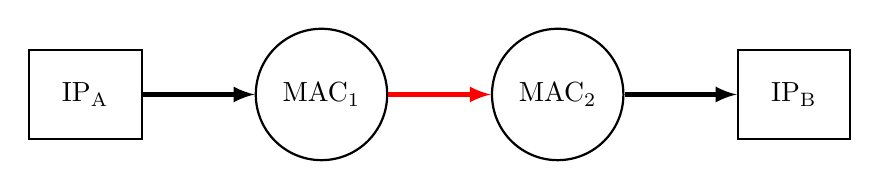
\begin{tikzpicture}
\node[IpNode](IPA) at (0,0) {IP\textsubscript{A}};
\node[MacNode](MAC1) at (3,0) {MAC\textsubscript{1}};
\node[MacNode](MAC2) at (6,0) {MAC\textsubscript{2}};
\node[IpNode](IPB) at (9,0) {IP\textsubscript{B}};

\draw[OpenEdge](IPA) -- (MAC1);
\draw[CloseEdge](MAC1) -- (MAC2);
\draw[OpenEdge](MAC2) -- (IPB);

\end{tikzpicture}
\caption[Flujo básico entre dos IPs]{Flujo básico entre IP\textsubscript{A} e IP\textsubscript{B}}
\label{fig:Analisis:BasicFlow}
\end{figure}

Este escenario nos deja con varias posibilidades que tenemos que tener en cuenta de manera especial: inserciones estándar de nuevos nodos en aristas abiertas, bifurcaciones y caminos huérfanos. De aquí en adelante se supondrá siempre el grafo en la situación de la Figura \ref{fig:Analisis:BasicFlow} como situación inicial. Decidiremos el caso en el que nos encontramos según la relación de las MACs origen y destino del nuevo paquete con las MACs ya introducidas en el grafo.

\subsection{Inserción estándar}
Una inserción estándar es aquella en la que simplemente estamos añadiendo información al grafo en alguna de las aristas abiertas. Sabemos que estamos en este caso cuando el nuevo paquete cumple una de estas dos condiciones:
\begin{itemize}
    \item La MAC origen coincide con la última MAC del grafo. Suponiendo la situación inicial y la llegada de un paquete con MAC origen igual a MAC\textsubscript{2} y MAC destino igual a MAC\textsubscript{3} se procede de la siguiente manera. Añadimos un nuevo nodo, MAC\textsubscript{3}, que se sitúa entre MAC\textsubscript{2} e IP\textsubscript{B}. Queda unido a  MAC\textsubscript{2} por una arista cerrada ya que hemos visto el salto físico y a IP\textsubscript{B} por una arista abierta ya que nos puede llegar más información. El resultado se muestra en el grafo de la Figura \ref{fig:Analisis:AddingLast}. El nodo añadido se muestra en color verde y las aristas nuevas en línea discontínua, se seguirá este convenio en el resto de grafos.
    \begin{figure}[H]
    \centering
    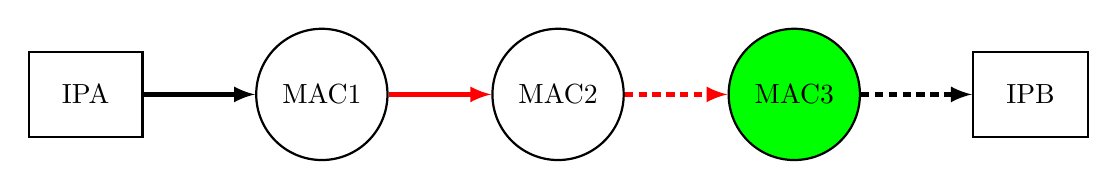
\begin{tikzpicture}
\node[IpNode](IPA) at (0,0) {IPA};
\node[MacNode](MAC1) at (3,0) {MAC1};
\node[MacNode](MAC2) at (6,0) {MAC2};
\node[NewMacNode](MAC3) at (9,0) {MAC3};
\node[IpNode](IPB) at (12,0) {IPB};

\draw[OpenEdge](IPA) -- (MAC1);
\draw[CloseEdge](MAC1) -- (MAC2);
\draw[NewCloseEdge](MAC2) -- (MAC3);
\draw[NewOpenEdge](MAC3) -- (IPB);
\end{tikzpicture}
    \caption[Ejemplo inserción básica 1]{Añadimos una nueva MAC al final del flujo}
    \label{fig:Analisis:AddingLast}
    \end{figure}
    \item La MAC destino coincide con la primera MAC del grafo. Suponiendo la situación inicial y la llegada de un paquete con MAC origen igual a MAC\textsubscript{0} y MAC destino igual a MAC\textsubscript{1} se procede de la siguiente manera. Añadimos un nuevo nodo, MAC\textsubscript{0}, que se sitúa entre IP\textsubscript{A} y MAC\textsubscript{1}. Queda unido a IP\textsubscript{A} por una arista abierta ya que nos puede llegar más información y a  MAC\textsubscript{2} por una arista cerrada ya que hemos visto el salto físico. El resultado se muestra en el grafo de la Figura \ref{fig:Analisis:AddingFirst}.
    \begin{figure}[H]
    \centering
    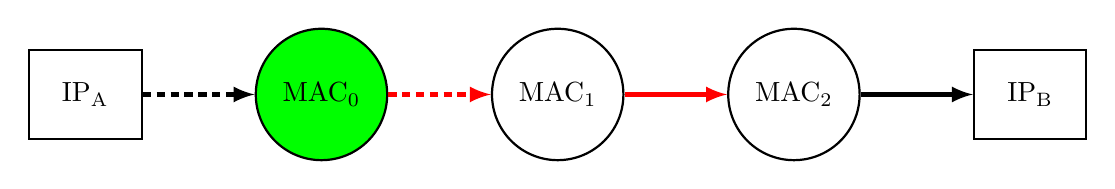
\begin{tikzpicture}
\node[IpNode](IPA) at (0,0) {IP\textsubscript{A}};
\node[NewMacNode](MAC0) at (3,0) {MAC\textsubscript{0}};
\node[MacNode](MAC1) at (6,0) {MAC\textsubscript{1}};
\node[MacNode](MAC2) at (9,0) {MAC\textsubscript{2}};
\node[IpNode](IPB) at (12,0) {IP\textsubscript{B}};

\draw[NewOpenEdge](IPA) -- (MAC0);
\draw[NewCloseEdge](MAC0) -- (MAC1);
\draw[CloseEdge](MAC1) -- (MAC2);
\draw[OpenEdge](MAC2) -- (IPB);
\end{tikzpicture}
    \caption[Ejemplo inserción básica 2]{Añadimos una nueva MAC al comienzo del flujo}
    \label{fig:Analisis:AddingFirst}
    \end{figure}
\end{itemize}
En ambos casos únicamente se añade información de un nodo y se cierra la arista correspondiente al salto físico que hemos visto. Utilizando esta operación de inserción básica podemos seguir añadiendo nodos MAC al flujo indefinidamente.

\subsection{Bifurcación}
Tanto en los flujos TCP como UDP, ambos manejados sobre IP, podemos encontrarnos con bifurcaciones en los caminos que recorren \cite{Priya}. Existen múltiples factores que pueden producir bifurcaciones en los flujos: caída temporal de una parte de la red, tareas de mantenimiento que inhabiliten un camino que se estaba usando, congestión de la red en sí. Estos son algunos ejemplos que provocan que los protocolos de transporte encargados de enviar los datos de una máquina a otra lo hagan por diversos caminos con tal de que lleguen. Esto tiene como consecuencia que nuestro grafo que conecta dos nodos IP puede ver estas bifurcaciones físicamente y tienen que quedar registradas como tal.

El modo de proceder para la inserción de una bifurcación será el siguiente. El estado inicial del grafo se corresponde con el camino que ya hemos visto y en un momento dado nos llega un paquete que ha pasado por un camino alternativo. Este es el caso de que alguna de las dos MAC del nuevo paquete se encuentre ya en nuestro grafo, pero no nos hallemos en ninguno de los casos anteriores. De esta manera, el nuevo nodo se insertará entre el nodo que ya está en el grafo y la IP correspondiente. Tendremos, entonces, dos maneras de llegar de IP\textsubscript{A} a IP\textsubscript{B}.

En el grafo de la Figura \ref{fig:Analisis:Bifurcation1} tenemos el resultado de añadir al grafo un paquete con MAC origen igual a MAC\textsubscript{1} y MAC destino igual a MAC\textsubscript{3}. Se observa que la única arista que se cierra es la que conecta MAC\textsubscript{1} con MAC\textsubscript{3} que se corresponde con el salto que hemos visto físicamente.
\begin{figure}[H]
\centering
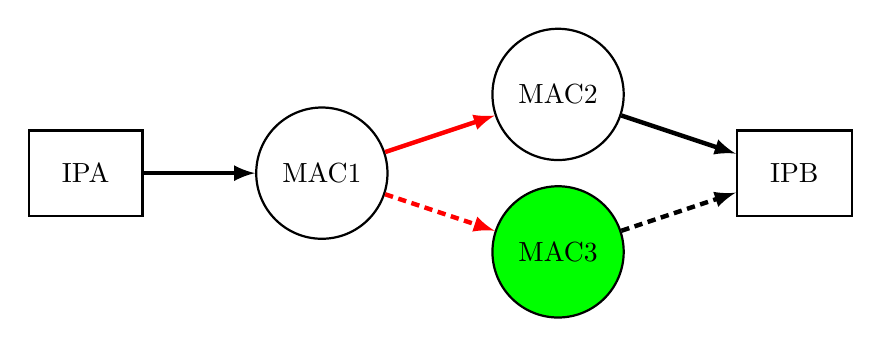
\begin{tikzpicture}
\node[IpNode](IPA) at (0,1) {IPA};
\node[MacNode](MAC1) at (3,1) {MAC1};
\node[MacNode](MAC2) at (6,2) {MAC2};
\node[NewMacNode](MAC3) at (6,0) {MAC3};
\node[IpNode](IPB) at (9,1) {IPB};

\draw[OpenEdge](IPA) -- (MAC1);
\draw[CloseEdge](MAC1) -- (MAC2);
\draw[NewCloseEdge](MAC1) -- (MAC3);
\draw[NewOpenEdge](MAC3) -- (IPB);
\draw[OpenEdge](MAC2) -- (IPB);
\end{tikzpicture}
\caption[Ejemplo de bifurcación 1]{Bifurcación al añadir paquete con MAC origen igual a MAC\textsubscript{1} y MAC destino igual a MAC\textsubscript{3}}
\label{fig:Analisis:Bifurcation1}
\end{figure}

Un caso similar ocurre si nos llegara un paquete con MAC origen igual a MAC\textsubscript{0} y MAC destino igual a MAC\textsubscript{2}. El procedimiento es homólogo al caso anterior y el resultado se puede observar en el grafo de la Figura \ref{fig:Analisis:Bifurcation2}
\begin{figure}[H]
\centering
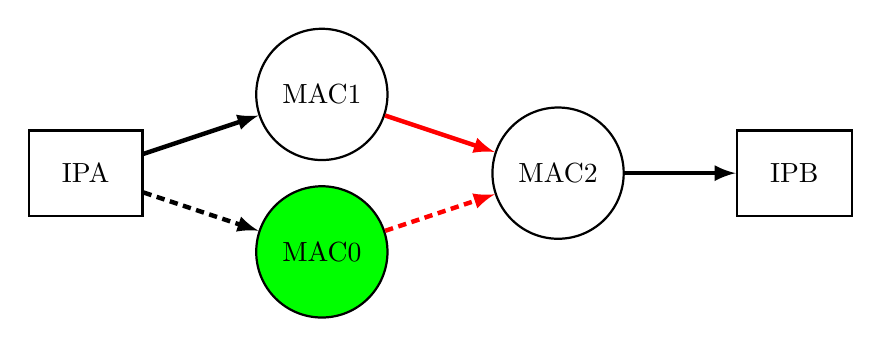
\begin{tikzpicture}
\node[IpNode](IPA) at (0,1) {IPA};
\node[NewMacNode](MAC0) at (3,0) {MAC0};
\node[MacNode](MAC1) at (3,2) {MAC1};
\node[MacNode](MAC2) at (6,1) {MAC2};
\node[IpNode](IPB) at (9,1) {IPB};

\draw[NewOpenEdge](IPA) -- (MAC0);
\draw[OpenEdge](IPA) -- (MAC1);
\draw[CloseEdge](MAC1) -- (MAC2);
\draw[NewCloseEdge](MAC0) -- (MAC2);
\draw[OpenEdge](MAC2) -- (IPB);
\end{tikzpicture}
\caption[Ejemplo de bifurcación 2]{Bifurcación al añadir paquete con MAC origen igual a MAC\textsubscript{0} y MAC destino igual a MAC\textsubscript{2}}
\label{fig:Analisis:Bifurcation2}
\end{figure}

%TODO: Ver si se añade esto aqui, como anexo o no se llega a añadir.
%Utilizando las dos maneras de insertar que se han descrito hasta el momento se puede llegar a cualquier grafo de los que describen un flujo entre dos IPs relacionado con MACs. Se propone un ejemplo en base al estado inicial añadiendo unos cuantos paquetes y observando como avanza el grafo. Se puede observar en la \fref{fig:Analisis:ComplexFlow}.

%\begin{figure}[h]
%%\centering
%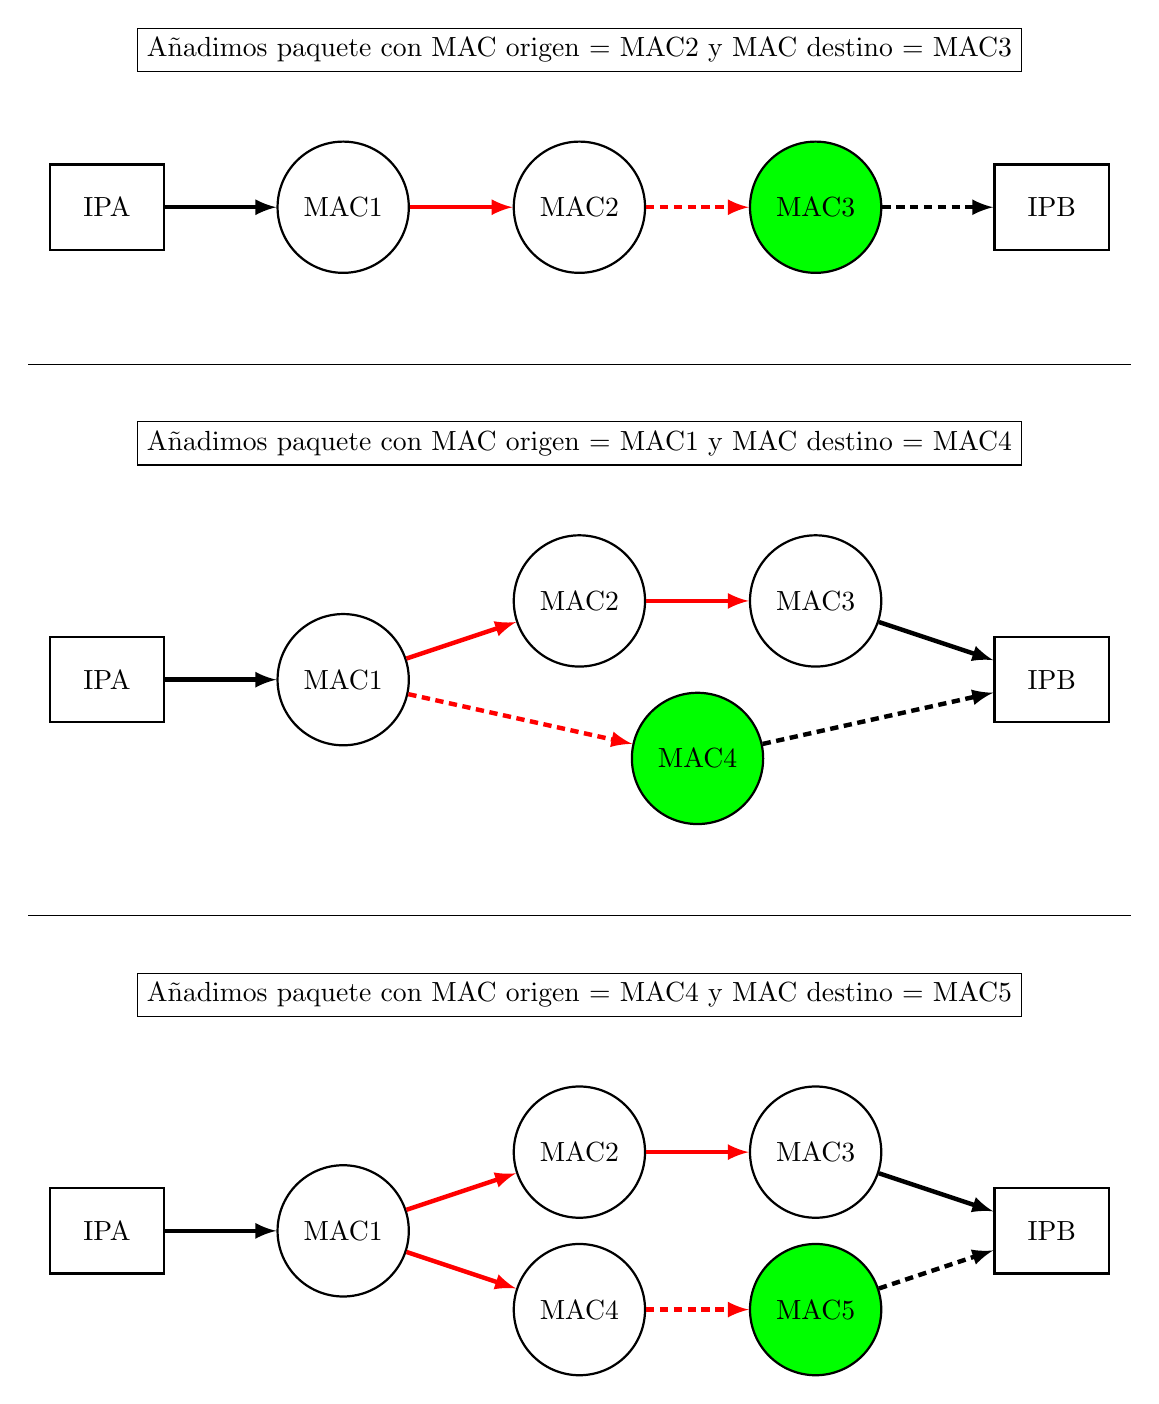
\begin{tikzpicture}
\node[draw] at (6,0) {Añadimos paquete con MAC origen = MAC2 y MAC destino = MAC3};

\node[IpNode](1IPA) at (0,-2) {IPA};
\node[MacNode](1MAC1) at (3,-2) {MAC1};
\node[MacNode](1MAC2) at (6,-2) {MAC2};
\node[NewMacNode](1MAC3) at (9,-2) {MAC3};
\node[IpNode](1IPB) at (12,-2) {IPB};

\draw[OpenEdge](1IPA) -- (1MAC1);
\draw[CloseEdge](1MAC1) -- (1MAC2);
\draw[NewCloseEdge](1MAC2) -- (1MAC3);
\draw[NewOpenEdge](1MAC3) -- (1IPB);

\draw (-1,-4) -- (13,-4);

%%%%%%%%%%%%%%%%%%%%%%%%%%%%%%%%%%%%%%%%%

\node[draw] at (6,-5) {Añadimos paquete con MAC origen = MAC1 y MAC destino = MAC4};

\node[IpNode](2IPA) at (0,-8) {IPA};
\node[MacNode](2MAC1) at (3,-8) {MAC1};
\node[MacNode](2MAC2) at (6,-7) {MAC2};
\node[NewMacNode](2MAC4) at (7.5,-9) {MAC4};
\node[MacNode](2MAC3) at (9,-7) {MAC3};
\node[IpNode](2IPB) at (12,-8) {IPB};

\draw[OpenEdge](2IPA) -- (2MAC1);
\draw[CloseEdge](2MAC1) -- (2MAC2);
\draw[NewCloseEdge](2MAC1) -- (2MAC4);
\draw[CloseEdge](2MAC2) -- (2MAC3);
\draw[OpenEdge](2MAC3) -- (2IPB);
\draw[NewOpenEdge](2MAC4) -- (2IPB);

\draw (-1,-11) -- (13,-11);

%%%%%%%%%%%%%%%%%%%%%%%%%%%%%%%%%%%%%%%%%%%%%%

\node[draw] at (6, -12) {Añadimos paquete con MAC origen = MAC4 y MAC destino = MAC5};

\node[IpNode](3IPA) at (0,-15) {IPA};
\node[MacNode](3MAC1) at (3,-15) {MAC1};
\node[MacNode](3MAC2) at (6,-14) {MAC2};
\node[MacNode](3MAC4) at (6,-16) {MAC4};
\node[MacNode](3MAC3) at (9,-14) {MAC3};
\node[NewMacNode](3MAC5) at (9,-16) {MAC5};
\node[IpNode](3IPB) at (12,-15) {IPB};

\draw[OpenEdge](3IPA) -- (3MAC1);
\draw[CloseEdge](3MAC1) -- (3MAC2);
\draw[CloseEdge](3MAC1) -- (3MAC4);
\draw[CloseEdge](3MAC2) -- (3MAC3);
\draw[NewCloseEdge](3MAC4) -- (3MAC5);
\draw[OpenEdge](3MAC3) -- (3IPB);
\draw[NewOpenEdge](3MAC5) -- (3IPB);
\end{tikzpicture}
%\caption[Ejemplo de superflujo compuesto]{Evolución del grafo tras añadir diferentes paquetes.}
%\label{fig:Analisis:ComplexFlow}
%\end{figure}

\subsection{Camino huérfano}
\label{subsec:Analisis:Reconstruccion:Huerfano}

Existe un caso particular en el que hay que prestar especial atención, los caminos huérfanos. Esta situación se da cuando el paquete que analizamos no tiene ninguna MAC incluida en el grafo. Llegados a este punto, no tenemos manera de saber en qué lugar colocar la nueva información que se nos da si no asumimos alguna condición más o extraemos más información del paquete aparte de sus direcciones IP y MAC. Se opta por la solución de extraer más información de los paquetes ya que estos incluyen muchos datos que no estamos usando y se evita asumir condiciones sobre la red. A estos datos que nos permitirán decidir el orden de nuevos nodos los llamaremos atributos de orden.

En concreto, los atributos de orden nos servirán para, dados dos nodos, saber cual se encuentra antes o después en el grafo y así poder insertarlo. Dado que recibimos la información en forma de paquetes, el valor de los atributos de orden dependerán exclusivamente del paquete que se estemos analizando. Dado que en el nuevo paquete sabemos que la MAC origen y destino están unidas por un salto físico (una arista cerrada en el grafo), el procedimiento consistirá en intentar insertar la MAC origen entre alguno de los nodos ya existentes. Tras esto el nodo correspondiente a la MAC destino se situará inmediatamente detrás. En el caso de que el paquete nuevo no pueda ser ordenado podemos proceder de dos maneras: guardar la información del paquete para volver a intentar insertarlo en un futuro cuando existan más nodos en el grafo o descartarlo, perdiendo así la información. Esta decisión se deja al desarrollo ya que, aunque guardar la información parece lo más correcto, puede ser un gasto ineficiente de memoria.

El atributo de orden que vamos a utilizar es el TTL de los paquetes. Es claro ver que, dados dos paquetes, podemos determinar que el que tenga un TTL mayor será el enlace que está antes en el flujo IP. Supongamos que nos encontramos en el estado inicial del grafo de la Figura \ref{fig:Analisis:BasicFlow} y que el paquete con los nodos de MAC\textsubscript{1} y MAC\textsubscript{2} tenía un TTL=64. En este punto, recibimos un paquete con MAC origen igual a MAC\textsubscript{3}, MAC destino igual a MAC\textsubscript{4} y TTL=63. Como ya hemos dicho, no tenemos una manera de introducir su información en el grafo, pero utilizando la información del TTL sabemos que este paquete está situado después de lo que ya teníamos. El estado del grafo quedaría como se observa en la Figura \ref{fig:Analisis:OrphanPath}.
\begin{figure}[H]
\centering
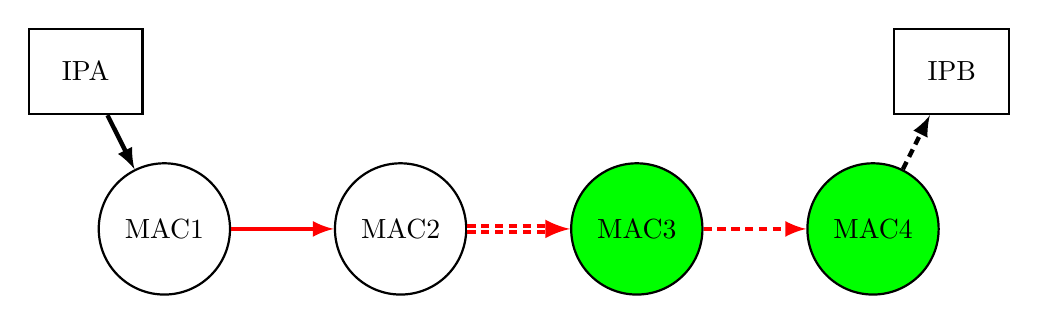
\begin{tikzpicture}
\node[IpNode](IPA) at (0,0) {IPA};
\node[MacNode](MAC1) at (1,-2) {MAC1};
\node[MacNode](MAC2) at (4,-2) {MAC2};
\node[NewMacNode](MAC3) at (7,-2) {MAC3};
\node[NewMacNode](MAC4) at (10,-2) {MAC4};
\node[IpNode](IPB) at (11,0) {IPB};

\draw[OpenEdge](IPA) -- (MAC1);
\draw[CloseEdge](MAC1) -- (MAC2);
\draw[NewVirtualEdge](MAC2) -- (MAC3);
\draw[NewCloseEdge](MAC3) -- (MAC4);
\draw[NewOpenEdge](MAC4) -- (IPB);
\end{tikzpicture}
\caption[Ejemplo de resolución de camino huérfano]{Insertamos el paquete huérfano gracias a la información del TTL.}
\label{fig:Analisis:OrphanPath}
\end{figure}

Cabe resaltar que la  arista entre MAC\textsubscript{2} y MAC\textsubscript{3} queda cerrada, pero es una arista especial en cuanto a que hemos inferido el salto entre MAC\textsubscript{2} y MAC\textsubscript{3} gracias a la información del TTL, es por esto que la marcaremos como arista virtual (arista con doble linea). Esto tendrá especial utilidad a la hora de detectar dispositivos.

\subsection{Problemas con la completitud de los flujos y el orden de los paquetes}
Un aspecto que sí que debe cumplir la traza que estamos analizando es una visión completa del flujo IP. Es necesario recoger información de todos los saltos para poder inferir de manera correcta el propio flujo. En trazas que abarquen el suficiente rango temporal, es complicado que no estemos viendo un flujo entre dos máquinas, en especial si estas se comunican frecuentemente. Dependiendo de nuestro objetivo final por el que estemos analizando la red puede ser útil observar trazas más o menos grandes. Por ejemplo, si simplemente queremos observar la topología de red, nos puede bastar con una traza pequeña. Con que se intercambie un paquete en cada salto la topología quedaría resuelta. Sin embargo, para analizar más en profundidad pérdida de paquetes u otros aspectos más específicos de la red necesitaremos trazas que abarquen más tiempo para garantizar su completitud.

Otro aspecto importante es el orden de los paquetes. La solución del problema propuesta no depende de que los paquetes se hallen ordenados para funcionar correctamente. De esta manera, si vemos un salto que es posterior en el flujo antes de tiempo puede quedar guardado como camino huérfano y ser insertado más adelante cuando llegue la información correspondiente. Dado que las capturas de tráfico se realizan a velocidades muy altas y dependiendo del programa que se utilice para capturar las trazas, no se puede asegurar que los paquetes que se muestran estén ordenados en entornos locales de pocos milisegundos. Al no depender del orden, estamos minimizando posibles errores relacionados con ello.

El único problema que podemos tener con el orden es a la hora de detectar \textit{firewalls}. Esto es debido a que, en muchos casos, los \textit{firewalls} no decrementan el TTL, viendo así dos paquetes con el mismo TTL pero con MACs origen y destino distintas respectivamente. Para solucionar este problema tenemos dos enfoques, cada uno con sus problemas. Podemos simplemente no detectar estos dispositivos, el salto que llegue antes se incluirá en el grafo y el otro se quedará como un camino huérfano que no se añadirá nunca. Esto tiene el problema de que no estamos detectando el flujo en su totalidad, lo que dará una salida errónea. La otra opción apuesta por introducir el \textit{firewall} al grafo, pero esto nos lleva al caso de estar comparando dos paquetes que tienen el mismo TTL. En este caso no tenemos ninguna manera que nos diga cual de los dos va antes, y es por esto que debemos asumir que los paquetes van a llegar en orden. Así, en la comparación de dos paquetes con el mismo TTL podremos decir que el que ha llegado más tarde se encuentra después en el grafo.

Finalmente, hemos tenido que optar por asumir que los paquetes se encuentran ordenados en la traza. Hemos mencionado que los programas de captura no pueden asegurar este orden, pero estos fallos ocurren con una frecuencia baja. Además, este tipo de suposición sobre el orden solo afecta a una parte muy pequeña del programa y no es necesario para la totalidad del funcionamiento. Se considera que la probabilidad de que los paquetes se hallen en desorden es baja, y que justo esto coincida con el momento que afecta a la solución propuesta es ínfimo. Por estos motivos la suposición es asumible y está basada en las fuentes de datos observadas.


\subsection{Relación entre el número de nodos y el número de aristas.}
\label{sec:Analisis:Edges per node}
A la hora de la implementación, será de especial utilidad el conocer cuál es la relación entre la cantidad de nodos y la cantidad de aristas que tiene nuestro grafo. Esto se utilizará más adelante para optimizar la eficiencia en memoria de nuestro programa. Para formalizar las conclusiones a las que se han llegado necesitaremos hacer uso de la siguiente notación:
\begin{align*}
	n =& \mathbin{\#}\{\textit{nodos en un grafo}\} \\
	a =& \mathbin{\#}\{\textit{aristas en un grafo}\} \\
	b =& \mathbin{\#}\{\textit{bifurcaciones en un grafo}\}
\end{align*}
Es claro ver que para un grafo sin bifurcaciones $a = n-1$, ya que todo nodo estará unido con el siguiente por una arista salvo el último. Por cada bifurcación, añadiremos al grafo un nodo y dos aristas, la que bifurca el nuevo camino y la que lo vuelve a unir, es decir, estamos añadiendo una arista de más. Nos es indiferente cuanto de largo sea el camino de una bifurcación ya que siempre se mantendrá la relación de que añadimos una arista por cada nodo. En conclusión, podemos afirmar que la relación entre el número de aristas y nodos es $$a = (n - 1) + b$$ Podemos ver el número de bifurcaciones por flujo IP como una variable aleatoria que depende de las características de cada red en específico. Por simplicidad, podemos decir que las bifurcaciones siguen una distribución de Poisson \cite{Spiegel}. Podemos entonces calcular el número de aristas esperadas en función de las bifurcaciones de la siguiente manera.
\begin{align*}
    \mathbb{E}(a) =&\ (n - 1) + \mathbb{E}(\bb Poisson(\lambda))\\
    \mathbb{E}(a) =&\ (n - 1) + \lambda \
\end{align*}
Para poder calcular el número de aristas necesitamos saber cuanto vale el parámetro $\lambda$. Para ajustar el modelo y estimar el parámetro $\lambda$, utilizaremos el método de estimación por máxima verosimilitud. Calculamos $\lambda = \widehat{\lambda} = \bar{b}$, siendo $\bar{b}$ la media muestral de bifurcaciones por flujo. Hay que tener en cuenta que, por las características de los grafos que utilizamos, los nodos IP no pueden tener bifurcaciones. En la \fref{tab:Analisis:Media bifurcaciones} se muestran los datos extraídos de empresas reales y los cálculos de la media muestral.
\begin{table}[hbtp]
	\centering
	\begin{tabular}{lccc}
		\toprule \textbf{Traza} & \textbf{Flujos IP}  & \textbf{Bifurcaciones} & \textbf{Media} \\ 
		\midrule
		Empresa 1 & 70.630 & 581 & 0,0082 \\
		Empresa 2 & 86.526 & 226 & 0,0026 \\
		Empresa 3 & 132.003 & 1.446 & 0,011 \\
		\textbf{TOTAL} & 289.159 & 2.253 & \textbf{0,0078} \\
		\bottomrule
	\end{tabular}
	\caption{Cálculo de la media muestral de bifurcaciones por flujo}
	\label{tab:Analisis:Media bifurcaciones}
\end{table}
Como podemos ver, la probabilidad de ocurrencia de una bifurcación es pequeña y dependiente de la red que se está analizando. Los resultados muestran que la media de bifurcaciones por $\bar{b} = 0,0078$. Aunque esta variación pueda parecer pequeña, hay que tener en cuenta que el número de flujos esperados es muy grande y esto hace que el ajuste tenga sentido. Por lo tanto nos queda como resultado final:
\begin{align*}
 \mathbb{E}(a) =&\ (n - 1) + 0,0078
\end{align*}

\section{Identificación de dispositivos en el superflujo}
\label{sec:Analisis:Dispositivos}
A lo largo de esta sección se describirán las soluciones que se plantean para la identificación de los distintos dispositivos que pueden aparecer en un flujo IP. Partimos del estado en el que ya se han analizado todos los paquetes que incluía la traza y se ha almacenado toda la información necesaria. El análisis pasa de recaer en cada flujo en particular a todos en su conjunto, de ahí que a partir de ahora los denominemos como superflujos.

El procedimiento que se seguirá ahora es deductivo. En primer lugar se llevará a cabo una identificación de dispositivos en general, sin diferenciar en tipos. Posteriormente, se clasificarán estos en función a una serie de reglas que se describen a lo largo de este capítulo.

\subsection{Identificación general de dispositivos}
Para determinar que existe un dispositivo en un punto concreto del grafo nos valdremos de haber usado anteriormente atributos de orden para la inserción de caminos. Como se ha visto en la sección \ref{subsec:Analisis:Reconstruccion:Huerfano}, cuando es posible ordenar un camino huérfano y lo insertamos dentro del grafo, se crea una arista virtual. Esto es debido a que su existencia ha sido inferida gracias a la información que encontramos en los paquetes, no a que la hayamos visto físicamente. Podemos deducir que estos saltos existentes que no vemos físicamente no son más que dispositivos de red que conectan la IP origen con la IP destino. Marcaremos todas estas aristas virtuales como dispositivos y se recopilarán las MAC\textsubscript{entrada} y MAC\textsubscript{salida} de cada uno. Estos dispositivos se guardan en un diccionario de dos claves, MAC\textsubscript{entrada} y MAC\textsubscript{salida}, respectivamente.

El problema que se plantea ahora es el de recopilar toda la información acerca de estos dispositivos; tanto para especificarla a la salida del programa, como para ayudarnos en la clasificación posterior. Tenemos una gran cantidad de dispositivos, que llamaremos dispositivos no resueltos dado que podemos observarlos como dispositivos separados aunque sean el mismo. Esto puede ocurrir, por ejemplo, si tenemos un \textit{router} con varias interfaces MAC y superflujos diferentes se conectan mediante interfaces diferentes. Es por esto que, mirando en el total de dispositivos, tendremos muchos repetidos y dependencias que podremos resolver simplemente agrupando los dispositivos por MAC de entrada y de salida vistas.

Para resolverlos, se utilizará un algoritmo recursivo que itera sobre todos los dispositivos individuales encontrados. Apoyándose en dos listas (\texttt{remain\_in\_macs} y \texttt{remain\_out\_macs}) resuelve las dependencias existentes entre las MAC\textsubscript{entrada} y MAC\textsubscript{salida}. Los dispositivos ya resueltos se van almacenando en la lista \texttt{devices}. El pseudocódigo puede verse en el Algoritmo \ref{lst:AlgoritmoResolucionDispositivos}
\begin{algorithm}[btp]
\begin{algorithmic}
\Function{resolve\_devices}{superflows}
\State unresolved\_devices $\gets$ \Call{detect\_devices}{superflows}

\ForAll{device \textbf{in} unresolved\_devices}
    \If{device[in\_mac] \textbf{is in} devices}
        \State break
    \EndIf
    \State new\_device $\gets$ \Call{device\_create}{\ }
    \State new\_device.in\_macs.\Call{append}{device.in\_mac}
    \State remain\_in\_macs $\gets$ \Call{create\_list}{\ }
    \State remain\_out\_macs $\gets$ \Call{create\_list}{\ }
    \State remain\_in\_macs.\Call{append}{device.in\_mac}
    \While{remain\_in\_macs \textbf{is not} EMPTY}
        \State mac $\gets$ remain\_in\_macs.\Call{pop}{\ }
        \ForAll{dev \textbf{in} unresolved\_devices \textbf{with} key1 == mac}
            \State new\_device.out\_macs.\Call{append}{device.out\_mac}
            \State remain\_out\_macs.\Call{append}{device.out\_mac}
        \EndFor
        \While{remain\_out\_macs \textbf{is not} EMPTY}
            \State mac $\gets$ remain\_out\_macs.\Call{pop}{\ }
            \ForAll{dev \textbf{in} unresolved\_devices \textbf{with} key2 == mac}
                \State new\_device.in\_macs.\Call{append}{device.in\_mac}
                \State remain\_in\_macs.\Call{append}{device.in\_mac}
            \EndFor
        \EndWhile
    \EndWhile
\EndFor

\EndFunction
\end{algorithmic}
\caption{Algoritmo de resolución de las dependencias de los dispositivos}
\label{lst:AlgoritmoResolucionDispositivos}
\end{algorithm}
El resto de la información relacionada con los dispositivos (bytes, \textit{frames} o VLANs) se va actualizando según se rellena la lista \texttt{devices}. Una vez identificados todos los dispositivos sin duplicidades podemos pasar a clasificarlos según su tipo.

\subsection{Clasificación de dispositivos}
El objetivo de la clasificación es la de diferenciar entre tres dispositivos diferentes: \textit{firewalls}, \textit{routers} y balanceadores de carga a nivel MAC. Una vez que tengamos todos los dispositivos agrupados y teniendo en cuenta la manera en la que detectamos dispositivos, clasificaremos como \textit{firewalls} todos aquellos que tenían decremento de TTL igual a 0. Esta decisión se toma en consecuencia con lo analizado en la sección \ref{subsec:Estado:Deteccion:Firewalls}, ya que tenemos en cuenta que los \textit{firewalls} intentan ser lo más transparentes posibles y no decrementaran el TTL de los paquetes que filtren.

Tras esto, nos quedan por clasificar balanceadores de carga y \textit{routers}. Como se explica en la sección \ref{subsec:Analisis:Dispositivos:Futuro}, en un futuro se podría añadir una clasificación más exacta y variada. Por el momento, nos limitaremos a clasificar los dispositivos restantes en balanceadores de carga a nivel MAC y los que no pasen el filtro serán identificados como \textit{routers}.

Para detectar los balanceadores de carga a nivel MAC, se utilizará un algoritmo simple (mostrado en Algoritmo \ref{lst:AlgoritmoDeteccionBalanceadores}) que mira las MACs de entrada y salida de los dispositivos quedándonos únicamente con las MACs \textit{unicast} y físicas. En el caso que veamos que se conectan más de una en alguno de los dos casos, podemos ver que se trata de un balanceador de carga a nivel MAC.
\begin{algorithm}[btp]
\begin{algorithmic}
\Function{detect\_load\_balancers}{devices}
\State valid\_in\_macs $\gets$ 0
\State valid\_out\_macs $\gets$ 0
\ForAll{device \textbf{in} devices}
    \ForAll{mac \textbf{in} device.in\_macs}
        \If{\Call{is\_unicast}{mac} \textbf{and} \Call{is\_physical}{mac}}
            \State valid\_in\_macs ++
        \EndIf
    \EndFor
    \ForAll{mac \textbf{in} device.out\_macs}
        \If{\Call{is\_unicast}{mac} \textbf{and} \Call{is\_physical}{mac}}
            \State valid\_out\_macs ++
        \EndIf
    \EndFor
    \If{valid\_in\_macs $\geq$ 2 \textbf{or} valid\_out\_macs $\geq$ 2}
        \State device.type $\gets$ LoadBalancer
    \Else
        \State device.type $\gets$ Router
    \EndIf
\EndFor
\EndFunction
\end{algorithmic}
\caption{Algoritmo de detección de balanceadores de carga a nivel MAC}
\label{lst:AlgoritmoDeteccionBalanceadores}
\end{algorithm}

\subsection{Futuros avances en clasificación}
\label{subsec:Analisis:Dispositivos:Futuro}
El proyecto propuesto en este TFG puede continuar ampliándose con nuevas funcionalidades relacionadas con la detección y clasificación de dispositivos. Durante el desarrollo del TFG se han planteado algunas que no se han desarrollado por diferentes motivos.

Un punto interesante para avanzar es la agregación de más información a nivel de dispositivo. Aunque en un principio la información se recopila a nivel de superflujo, es interesante también recopilar la información a nivel de dispositivo aunque haya información duplicada. El número de dispositivos que veremos no escala con respecto al tamaño de los archivos analizados ya que no aparecen más. Información útil a nivel de dispositivo puede ser las IPs de entrada y de salida con vistas a analizar las subredes que conecta.

Otro avance que se podría dar en el futuro es una clasificación más estricta y variada. Los balanceadores de carga a nivel IP serán un paso natural una vez que se realice la agregación propuesta en el párrafo anterior. Además, existen maneras conocidas no solo para la clasificación de balanceadores usuales, sino para disgregar entre \textit{routers} estándar y \textit{routers} que estén realizando un proceso NAT.

\chapter{Estructura y desarrollo}
\label{chap:Desarrollo}
A lo largo de este capítulo se describen en detalle las decisiones que se han tomado durante el desarrollo de la aplicación. Se analiza como se ha integrado la solución propuesta en aprovechando un proyecto ya existente, \textit{fisher}, que elementos de este se han usado y cuales se han modificado. Además, se habla sobre las entradas que soporta el programa y que salidas ofrece.

\section{Decisiones generales de desarrollo}
La primera parte del desarrollo consistió en implementar el módulo de reconstrucción de caminos. Esto se realizó como parte de un programa más amplio llamado \textit{fisher}, desarrollado por Guillermo Julián como programa interno para Naudit. Se decidió utilizar C como lenguaje de desarrollo por las características del proyecto. Uno de los problemas que se encontró en el anterior intento de desarrollar un programa similar en Python fue la lentitud del mismo, en especial en archivos de gran tamaño. Lo que nos permite C es gestionar la memoria a un nivel más bajo, con lo que podemos realizar los mismos procesos que con otros lenguajes de más alto nivel, pero con una mayor eficiencia. Se pretende que con este cambio en el lenguaje de desarrollo se lleguen a las velocidades esperadas en el análisis así como a una mayor eficiencia en memoria.

Como se ha mencionado, el desarrollo se centro en ampliar la funcionalidad de \textit{fisher}. Dicha aplicación se centraba en el análisis de trazas pcap mediante la definición de funciones que se encargan de la inicialización, pre-procesado, análisis, post-procesado y salida de los registros de la traza pcap. Se disponen de diferentes lectores de trazas (NDLeeTrazas, lpcap, mmpcap y hpcap), en general se usará NDLeeTrazas por defecto ya que es el más versátil en cuanto a formatos de traza que se utilizaran en el futuro. 
%(Guillermo) En este caso NDLeeTrazas es el más versátil en cuanto a formatos de traza y uso (lpcap usa la librería libpcap así que va lento, mmpcap hace un mmap del fichero entero en memoria antes de leer, y hpcap lee directamente del driver). No sé si hace falta mencionar todo esto (quizás con decir que NDLeeTrazas es el que soporta los formatos que nos interesan vale) pero te lo pongo aquí para que lo sepas, por si te lo preguntan.
Se han utilizado y modificado varias de las librerías de este programa, haciéndose uso de facilidades como el log, utilidades para estructuras IP y MAC, el gestor de memoria para generar \textit{pools} de memoria o la estructura de tests ya desarrollada para garantizar la funcionalidad del código escrito.

En un comienzo se pensó que con el análisis de trazas pcap sería suficiente. Sin embargo, se consideró que sería útil que fuera posible realizar el análisis de superflujos a partir de otros ficheros de origen. No siempre se iba a disponer de la traza pcap en bruto y el módulo de análisis de superflujos tiene la flexibilidad suficiente para adaptarse a diferentes tipos de entrada que le aporten más o menos información. El ejemplo más claro fue el de la salida de \textit{Procesa} un programa interno que lee y extrae información del tráfico de red y la presenta como registros por flujo. El programa ha quedado modularizado para que la incorporación de nuevos tipos de archivos de entrada sea cómoda y rápida.

El desarrollo del módulo completo de análisis de superflujos ha supuesto para \textit{fisher} un aprovechamiento de su potencial y una ampliación de su funcionalidad. Como se ha especificado, fisher es un programa centrado en el procesamiento de trazas pcap; fue por esto que se considero la implementación del analizador de superflujos como una parte de este programa. Más adelante, se añadieron nuevas funcionalidades acordes a las necesidades específicas del proyecto, como fue el análisis de la salida de Procesa además de la de trazas pcap.

\section{Librerías usadas pertenecientes a fisher}
Durante el desarrollo del módulo de análisis de superflujos se aprovechó el código ya escrito de \textit{fisher} y la estructura interna del programa para facilitar el manejo de estructuras, el análisis de fallos y las pruebas de código. Las librerías de las que se hizo uso directo se enumeran a continuación y se describe el uso que se dio de cada una:
\subsection{Types y errors}
Librerías básicas con definiciones de macros que se usaron para que el módulo implementado fuera coherente con el resto del programa. Facilitan el control de errores internos ya que mantienen la misma estructura de errores y la legibilidad del código.
\subsection{Log} 
Librería para el manejo de la información del flujo del programa durante su ejecución. Dispone de diferentes niveles de profundidad que se pueden seleccionar al ejecutar y que muestran más o menos información dependiendo de lo que se desee. Útil para distinguir en el log entre errores más graves y consideraciones solo usadas para la depuración de código.
\subsection{Static mem}
Librería para la gestión de la memoria estática. Evitar el uso de reservas de memoria continuamente fue uno de los requisitos exigidos para el desarrollo del módulo. Se consideró que la gestión dinámica de memoria mediante las funciones estándar de C (malloc y free) era muy lenta dado la cantidad de estas reservas que habría que hacer. Es por esto que la gestión se dejo a una librería ya desarrollada. 

Conceptualmente lo que se realiza es solo una reserva de memoria mediante la función malloc en la que, mediante la librería \texttt{static\_mem}, se definía la cantidad total de entidades de un mismo tipo de estructura se van a reservar a lo largo de la ejecución del programa. Esto conlleva realizar un \textit{pool} diferente para cada tipo de estructura, pero resulta en una mejora en la eficiencia general del programa.
\subsection{Funciones de utilidad para estructuras IP y MAC}
Estas librerías ya existentes fueron modificadas incluyendo nuevas funciones que eran necesarias para el uso de la librería de lista de capas que se desarrolló para manejar los grafos. Las funciones que ya se incluían eran comparadores, copiadores y conversores a cadenas de caracteres tanto de estructuras IP como MAC. Estas funciones son las que se pasan como punteros al programa para que los nodos del grafo fueran lo mas abstractos posible. También las estructuras de listas y diccionarios hacen uso de estas funciones.
\subsection{\textit{Packet parser}}
Librería con las funciones necesarias para leer la información del paquete a nivel de byte y pasarla a una estructura manejable por el programa. También se amplió la funcionalidad de esta librería introduciendo la extracción de la información a nivel MAC y la extracción de las opciones dentro de la capa TCP.
\subsection{Tests}
Como parte de \textit{fisher}, se disponía de un módulo totalmente automatizado para realizar pruebas y comprobar la funcionalidad del código. Se hizo uso de esta posibilidad para tener tests unitarios que aseguraran el funcionamiento básico de la librería principal que almacenaba el grafo y, más adelante, del análisis de trazas y la detección de dispositivos. Esto hizo que se pudiera comprobar con mucha facilidad el funcionamiento correcto del programa, así como localizar los errores de manera sencilla. Se describen los tests realizados con más detalle en la sección \ref{chap:Pruebas:Test}
\subsection{Estructuras de listas y diccionarios}
Dentro de \textit{fisher} se contaba con algunas estructuras de datos ya implementadas. En concreto, se hizo uso de las listas y de los diccionarios simples y de dos claves. En este último caso, se realizaron modificaciones para evitar el uso excesivo de mallocs en el post-procesado y aprovechar una vez más la libreria \texttt{static\_mem}.

\section{Módulo de ordenación de superflujos}
Este módulo encargará de la inserción de nuevos elementos a los superflujos, manteniendo el orden, respetando la información perteneciente a cada capa (MAC o IP) y actualizando la información tanto de nodos como de aristas. Además, tendrá en cuenta los atributos de orden que se le indiquen para inferir el lugar de los nodos que no puedan ser reconocidos directamente. Guarda también información de nodos que no se puedan insertar por sus características, para que en otro momento de la ejecución se puedan volver a intentar insertar.

\subsection{Estructura de datos usada}
A un nivel abstracto, este módulo representa un grafo orientado con un único nodo inicial y un único nodo final, el propuesto en la solución y que guarda la información de cada superflujo. Cada nodo puede pertenecer a una de las capas que se indican al inicializar la estructura y puede comunicarse con nodos de su misma capa o de las adyacentes. En el caso de superflujos las capas serán IP y MAC. Para la implementación de este módulo se han creado 5 estructuras que se relacionan entre ellas. Se describen a continuación:
\begin{itemize}
    \item Lista de capas: Es la estructura general donde se almacena la información de la lista y se definirá una por cada superflujo. En su inicialización se debe indicar: los \textit{pools} de memoria para los nodos y las aristas, la información de cada capa, su orden y el número de estas, el número de atributos de orden y las funciones para actualizarlos y usarlos para ordenar nodos y la función que pasa de la estructura de donde se sacará la información de cada camino a la estructura de camino en sí. Una vez definida e inicializada una estructura de lista de capas, se puede insertar caminos estandarizados con la función (\texttt{parse\_to\_path}), que ha tenido que ser previamente definida, simplemente llamando a la función \texttt{layer\_list\_add\_path}. Aparte de esto guarda información sobre los caminos huérfanos y el inicio del grafo.
    \item Información de capa: Se guarda la información relacionada con cada capa. Se define de manera global para los nodos de tipo IP y MAC ya que todos comparten la misma información respecto a la capa. Así, cada nodo únicamente tiene un puntero a la estructura de información de su capa y la eficiencia de memoria usada es mayor. La información que se almacena es: funciones para comparar, copiar y pasar a cadena de caracteres elementos de la capa, así como el \textit{pool} de memoria.
    \item Nodos de la lista: Se define uno por cada nodo que se intenta insertar en el grafo y se libera memoria en los que ya se ha extraído toda la información necesaria. De esta manera, quedan únicamente definidos hasta la finalización del programa los que han sido añadidos al grafo y los nodos pertenecientes a caminos huérfanos.  En los nodos se almacena información sobre el elemento, los atributos de orden de ese nodo y las siguientes aristas que conectan este nodo con el resto del grafo.
    \item Aristas: No se definen hasta que no se insertan los nodos que conectan en la lista. Guardan la información de las aristas (VLANs, paquetes, bytes, RTT) que se va actualizando al añadir nuevos caminos y el tipo de conexión que establece entre nodos (real, virtual o cambio de capa).
    \item Caminos: Esta estructura es el enlace entre estructuras exteriores al módulo y las que pertenecen. Es necesaria para mantener la cohesión y el correcto comportamiento del resto de funcionalidades. Por lo tanto, se define un camino por cada paquete que estamos analizando. Es en la función \texttt{parse\_to\_path} donde se debe rellenar la información necesaria de esta estructura en función de los datos que se consideren convenientes. En el caso más general se rellenaran con los datos de un paquete.
\end{itemize}

\subsection{Algoritmo para ordenar cada camino del superflujo}
El grafo ordenado representa los diferentes caminos que puede seguir un paquete para llegar desde el nodo de inicio hasta el nodo final. Dependiendo de la red, el número de capas y la longitud de los caminos vistos la complejidad de estos grafos puede variar. En el caso más general intervendrán únicamente dos capas (IP y MAC) y la longitud de los caminos es de 4 (Nodo IP -> Nodo MAC -> Nodo MAC -> Nodo IP). Asumiendo esto nos servirá de ejemplo para la explicación del algoritmo de inserción y ordenación de caminos.

Partimos de una lista por capas inicializada, en la que aún no se han insertado caminos. Por cada información de camino que nos llegue, se llamará a la función \textit{parse\_to\_path} para pasar a una estructura estándar que entienda la función \textit{layer\_list\_add\_path}. Una vez dentro de esta función, miramos que nodos del nuevo camino se encuentran en el grafo. Cobran especial relevancia el último nodo del nuevo camino que ya esté en el grafo antes de encontrar un nodo que no esta en el grafo y el primer nodo del nuevo camino que ya está en el grafo después de encontrar nodos que no están en el grafo. Entre estos dos se encontrará la información nueva que podemos introducir en el grafo.

Tenemos cuatro escenarios en función de los valores de estas dos variables:
\begin{itemize}
    \item Si todos los nodos del nuevo camino ya se encontraban en el grafo tenemos un \textbf{camino repetido}. En este caso actualizamos la información de los nodos y aristas repetidos.
    \item Si los únicos nodos del nuevo camino que se encuentran en el grafo son el primero y el último, entonces tenemos un \textbf{camino huérfano}. En este caso intentamos ordenarlo en base a los atributos de orden.
    \begin{itemize}
        \item Si conseguimos ordenarlo, lo insertamos en el grafo actualizamos la información de los nodos y aristas repetidas.
        \item Si no se puede ordenar, lo añadimos a la lista de caminos huérfanos.
    \end{itemize}
    \item Si los nodos del nuevo camino que conocemos no son adyacentes en el grafo tenemos una \textbf{bifurcación}. Añadimos los nuevos nodos al grafo y actualizamos la información de los nodos y aristas repetidas.
    \item Si no es ninguno de los casos anteriores tenemos una \textbf{inserción estándar}. Insertamos los nuevos nodos en el grafo y actualizamos la información de los nodos y aristas repetidas.
\end{itemize}
Tras cada inserción exitosa, se realiza una pasada por los caminos huérfanos acumulados para ver si es posible ordenarlos ahora con la nueva información recabada.

\subsection{Estructura de funciones y submódulos}
\label{subsec:Desarrollo:Ordenacion:EstructuraFunciones}
El desarrollo del analizador de superflujos y la posterior identificación y clasificación de dispositivos se ha diseñado y estructurado en lo que podríamos llamar submódulos con funcionalidades identificadas y diferenciadas. La intención de esto es poder facilitar el desarrollo y la ampliación futura del programa. Además, esto simplifica la detección de errores y su resolución y ayuda a comprender el código a personas externas al desarrollo en caso de ser necesario.
\begin{figure}[H]
\centering
\makeatletter

\pgfdeclareshape{document}{
\inheritsavedanchors[from=rectangle] % this is nearly a rectangle
\inheritanchorborder[from=rectangle]
\inheritanchor[from=rectangle]{center}
\inheritanchor[from=rectangle]{north}
\inheritanchor[from=rectangle]{south}
\inheritanchor[from=rectangle]{west}
\inheritanchor[from=rectangle]{east}
% ... and possibly more
\backgroundpath{% this is new
% store lower right in xa/ya and upper right in xb/yb
\southwest \pgf@xa=\pgf@x \pgf@ya=\pgf@y
\northeast \pgf@xb=\pgf@x \pgf@yb=\pgf@y
% compute corner of ‘‘flipped page’’
\pgf@xc=\pgf@xb \advance\pgf@xc by-10pt % this should be a parameter
\pgf@yc=\pgf@yb \advance\pgf@yc by-10pt
% construct main path
\pgfpathmoveto{\pgfpoint{\pgf@xa}{\pgf@ya}}
\pgfpathlineto{\pgfpoint{\pgf@xa}{\pgf@yb}}
\pgfpathlineto{\pgfpoint{\pgf@xc}{\pgf@yb}}
\pgfpathlineto{\pgfpoint{\pgf@xb}{\pgf@yc}}
\pgfpathlineto{\pgfpoint{\pgf@xb}{\pgf@ya}}
\pgfpathclose
% add little corner
\pgfpathmoveto{\pgfpoint{\pgf@xc}{\pgf@yb}}
\pgfpathlineto{\pgfpoint{\pgf@xc}{\pgf@yc}}
\pgfpathlineto{\pgfpoint{\pgf@xb}{\pgf@yc}}
\pgfpathlineto{\pgfpoint{\pgf@xc}{\pgf@yc}}
}
}
\makeatother

\tikzstyle{Input}=[shape=document, draw=black, fill=palette1, thick, align=center, opacity=.8, text opacity=1, draw opacity=1, minimum width=15mm, minimum height=20mm]
\tikzstyle{Module}=[rectangle, draw=black, fill=palette2, thick, inner sep=10pt, align=center, opacity=.8,text opacity=1, draw opacity=1]
\tikzstyle{Library}=[rounded corners, draw=black, fill=palette3, thick, inner sep=7pt, align=center, opacity=.8,text opacity=1, draw opacity=1]
\tikzstyle{Output}=[shape=document, draw=black, fill=palette4, thick, inner sep=7pt, align=center, opacity=.8,text opacity=1, draw opacity=1, minimum width=15mm, minimum height=20mm]
\tikzstyle{connection}=[->, line width=1mm, draw=black]
\tikzstyle{double connection}=[<->, line width=1mm, draw=black]


\begin{tikzpicture}
\begin{scope}

%\node[anchor = north] at (1.5, -6.5) {\textit{fisher}};
\fill[dashed, palette5, opacity=.5, draw opacity=1,  draw=black, ultra thick] (1.5, 2) rectangle (11, -6.5);

\node[Input](pcap) at (0,0) {Traza\\ pcap};
\node[Input](procesa) at (0,-3) {Fichero\\ \textit{Procesa}};
\node[Module](sfpcap) at (3.2,0) {Módulo\\ PCAP};
\node[Module](sfprocesa) at (3.2,-3) {Módulo\\ \textit{Procesa}};
\node[Module](sfipmac) at (7.5,-1.5) {Módulo\\ IPMAC};
\node[Library](layerlist) at (6, -5) {Librería\\ ordenación\\ superflujos};
\node[Library](devicesdetection) at (9, -5) {Librería\\ detección\\ dispositivos};
\node[Output](superflows) at (13, 0) {Salida\\superflujos\\ (registros)};
\node[Output](devices) at (13, -3) {Salida\\ dispositivos\\ (json)};

\draw[connection] (pcap.east) -- (sfpcap.west);
\draw[connection] (procesa.east) -- (sfprocesa.west);
\draw[connection] (sfpcap.east) -- (sfipmac.west);
\draw[connection] (sfprocesa.east) -- (sfipmac.west);
\draw[connection] (sfipmac.east) -- (superflows.west);
\draw[connection] (sfipmac.east) -- (devices.west);
\draw[double connection] (sfipmac.south) -- (layerlist.north);
\draw[double connection] (sfipmac.south) -- (devicesdetection.north);

\end{scope}
\end{tikzpicture}
\caption[Flujo del programa]{Flujo de ejecución del programa}
\label{fig:Desarrollo:Flujo del programa}
\end{figure}
Como se puede ver en la Figura \ref{fig:Desarrollo:Flujo del programa} el flujo del programa comienza dependiendo de la entrada que se seleccione, pudiendo ser esta una traza \textit{pcap} o un fichero de registros proveniente de \textit{Procesa}. Tras esto, los respectivos módulos se encargarán de facilitar la comunicación entre sus ficheros de entrada y el módulo de IP/MAC (que se explicará en detalle en \ref{sec:Desarrollo:IPMAC}). Con respecto al flujo del programa, el módulo IP/MAC es el que más carga tiene, ya que se encarga de las llamadas a la librería \texttt{layer\_list} (que contiene la funcionalidad de almacenar el grafo de superflujos y ordenarlo) y posteriormente de la identificación y clasificación de dispositivos llamando a la librería \texttt{device\_detection} (encargada de la detección y clasificación de dispositivos). La inicialización y destrucción de las estructuras necesarias para el funcionamiento del proceso también son responsabilidad de este módulo.

Se generan dos ficheros de salida tras la ejecución del programa. El primero de ellos contiene la información correspondiente a los superflujos, sus conexiones y parámetros. Está en forma de registros a nivel de un registro por arista del grafo. El segundo recoge la información correspondiente a los dispositivos, su tipo y parámetros recopilados. Este es un fichero JSON con todos los detalles de cada dispositivo. A partir de estos ficheros se puede utilizar la información por otros programas teniendo en cuenta el formato que presenta y que queda definido en la documentación del código.

\section{Módulo de superflujos IP/MAC}
\label{sec:Desarrollo:IPMAC}
Este módulo utiliza directamente todas las estructuras y funcionalidades del módulo de ordenación de superflujos. Se realiza de manera abstracta para que se pueda seleccionar la estructura de entrada de donde se sacará la información para los nodos y aristas del grafo ordenado. En este módulo se fijan la inicialización de las estructuras necesarias para el análisis de superflujos, la adición de nuevos caminos al grafo y la salida que genera el programa. Se comentan los aspectos más relevantes de este módulo.

\subsection{Calculo de coeficientes para la reserva de los \textit{pools} de memoria}
\label{subsec:Desarrollo:IPMAC:CoefPools}
El programa esta capacitado para usar solo la memoria que se considere necesaria en el momento de la ejecución (por defecto es 32 MB) para las estructuras que se encargan de la ordenación de los superflujos. Como se ha comentado anteriormente, se tiene que definir un \textit{pool} de memoria diferente para cada estructura y definir cuantas de estas estructuras se van a querer reservar concurrentemente como máximo. Las estructuras para las que es necesario definir un \textit{pool} de memoria son: superflujos, nodos de grafo, aristas de grafo, elementos IP y elementos MAC.

\begin{table}[hbtp]
	\centering
	\small
	\begin{tabular}{lcc}
		\toprule \textbf{Estructura} & \textbf{Número de estructuras}  & \textbf{Número de estructuras por superflujo} \\ \midrule
		Superflujos & s & 1 \\
		Elementos IP & i & 2 \\
		Elementos MAC & m & $\alpha$ \\
		Nodos & n & $i + m = 2 + \alpha$ \\
		Aristas & a & $(n - 1) + \lambda$  \\ \bottomrule
	\end{tabular}
	\caption{Coeficientes de reserva de memoria por cada superflujo}
	\label{tab:Desarrollo:Coeficientes memoria}
\end{table}

La manera de estimar el número de estructuras que reservar de cada tipo se basa en que por cada superflujo podemos estimar la cantidad de los demás elementos que necesitamos en promedio. Esto se traduce en unos coeficientes que se pueden ver en \fref{tab:Desarrollo:Coeficientes memoria}. Es claro que por cada superflujo habrá 2 elementos IP (IP origen e IP destino) y que el número de nodos será la suma de los elementos IP y los elementos MAC. Existen dos casos especiales: el promedio de MACs por superflujo y el promedio de aristas por superflujo.

Para estos dos casos se ha recurrido a la observación en casos experimentales. Hay que resaltar que estos parámetros son variables y que se pueden ajustar en función de las características específicas de cada red. En la \fref{sec:Analisis:Edges per node} se razonó el valor tomado para $\lambda$. Para el calculo del parámetro $\alpha$ se recurre a la observación en trazas reales. En la tabla \ref{tab:Pruebas:Ratios estructuras} puede comprobarse como se realiza ese cálculo.

Conociendo el tamaño de memoria del que disponemos para nuestras estructuras así como el tamaño de cada una (denotado como $x_{tam}$) podemos conocer cual es la manera óptima de repartir la memoria. Utilizando los superflujos como unidad de memoria (denotada como $u$) podemos obtener la cantidad de unidades de memoria que podemos reservar de esta manera.

$\begin{array}{lcl}
	\mathrm{memoria} & = & s \cdot s_{tam} + i \cdot i_{tam} + m \cdot m_{tam} + n \cdot n_{tam} + a \cdot a_{tam}\\
	\mathrm{memoria} & = & u \cdot s_{tam} + 2u \cdot i_{tam} + \alpha u \cdot m_{tam} + (2u+\alpha) \cdot n_{tam} + \beta \cdot a_{tam} \\
	u & = & \frac{\mathrm{memoria}}{s_{tam} + 2 \cdot i_{tam} + \alpha \cdot m_{tam} + (2u+\alpha) \cdot n_{tam} + \beta \cdot a_{tam}}
\end{array}$

Y de esta manera podemos calcular cuantas estructuras reservar de cada tipo en función de la unidad de memoria elegida, que en este caso es el número de superflujos.

$\begin{cases}
	s = u\\ 
	i = 2u\\ 
	m = \alpha u\\
	n = (2+\alpha)u\\
	a = (n - 1 + \lambda) u
\end{cases}$

\subsection{Salida del programa}
El programa tiene diferentes tipos de salida que se pueden elegir en función de las necesidades específicas de cada momento. Se dispone de una salida por consola que muestra el estado del análisis de superflujos durante la ejecución y un resumen de los superflujos y dispositivos que se han encontrado. Dependiendo del tamaño de la traza que vayamos a analizar esta salida por consola puede resultar útil o excesiva. Mediante los comandos \texttt{--extra-info}, para una información aún más detallada y \texttt{--no-console-output}, para desactivarla; el usuario puede ajustarlo en cada ejecución.

La información recopilada se almacena en dos archivos de salida, uno para la información de superflujo y otro para la información de los dispositivos. El primero contiene registros de los grafos de cada superflujo, un registro por cada arista con la información de los nodos que conecta. El fichero de salida de los dispositivos será en formato JSON dado que una estructura de registros no se acomodaba tanto a las características de estos. El número de MACs, VLANs o IPs que se conectan es variable y la posterior lectura de un archivo de registros en este formato podría ser tediosa. Por este motivo se eligió el formato JSON, más estructurada y que se adapta más las necesidades en este caso.

\section{Identificación de los elementos de red}
Como ya se describió en la sección \ref{sec:Analisis:Dispositivos} posteriormente a la ordenación de superflujos y una vez que se ha procesado toda la traza se tratarán de identificar los dispositivos y clasificarlos. En esta sección se comentan los aspectos relevantes que surgieron durante el desarrollo de esta parte del proyecto.

\subsection{Identificación general de dispositivos}
La identificación de dispositivos se corresponde con el postprocesado dentro de la estructura de funciones que se ha desarrollado. Consiste simplemente en seguir el algoritmo \ref{lst:AlgoritmoResolucionDispositivos} con las consideraciones usuales para el lenguaje de programación C. Las estructuras correspondientes a almacenar la información de dispositivos se declaran en el módulo IP/MAC, haciéndolo así abstracto a la entrada que se elija. Las funciones, aunque pertenecientes al mismo módulo, se sitúan en un fichero diferente para así tenerlas localizadas de una manera más sencilla y facilitar las pruebas que se realizaron.

Es importante mencionar que en esta parte del desarrollo no se ha usado la librería \texttt{static\_mem} ya que el número de dispositivos no escala linealmente con el tamaño de la traza y llega un punto en el que se mantiene estable. Es por esto que los tiempos de ejecución no son tan altos y no era necesario su uso. De lo que si se ha hecho uso es de los diccionarios de una y dos claves que ya estaban implementados en \textit{fihser}. Concretamente, el diccionario de dos claves ha sido de especial utilidad para la resolución de los dispositivos, ya que nos permitía iterar por cualquiera de las dos claves (MAC\textsubscript{entrada} y MAC\textsubscript{salida} en nuestro caso).

\subsection{Clasificación de dispositivos}
La clasificación de dispositivos se realiza en dos pasos: primero identificamos los \textit{firewalls} y después los balanceadores de carga a nivel MAC. Los elementos que no queden clasificados en ninguno de los dos casos se identificarán como \textit{routers} a falta de añadir más elementos a clasificar en un futuro.

Como se dispone de los atributos de orden, se debe de especificar al módulo IP/MAC cuál de ellos se corresponde con el TTL para poder realizar la detección de elementos de red. En el caso de no indicarse, simplemente el postprocesado no se ejecutará y la detección de dispositivos no se realizará. Los dispositivos con un TTL = 0 se clasifican como \textit{firewalls} directamente, y se sigue el algoritmo \ref{lst:AlgoritmoDeteccionBalanceadores} para diferenciar entre balanceadores de carga y \textit{routers}.

Una vez que hecho esto, el programa finaliza especificando todo el análisis en los dos ficheros de salida. La clasificación de dispositivos no se considera finalizada aunque si funcional. Esto significa que se puede ampliar con relativa facilidad añadiendo nuevas reglas o haciendo más estrictas las existentes para desgranar en mayor medida los dispositivos que se detectan.


\section{Diferentes tipos de entradas}
El programa de análisis de superflujos se ha diseñado pensando principalmente para el análisis de trazas \textit{pcap}, debido a que el propio \textit{fisher} del que forma parte está desarrollado para su análisis. Sin embargo, se dio la situación en la que se pudieran utilizar otro tipo de archivos internos como entrada. En estos casos, hay que indicar mediante un programa que sirva de enlace entre el formato de entrada y la libreria \texttt{superflows\_ipmac}. A continuación se describen los tipos de entrada que han quedado implementados.

\subsection{Trazas pcap}
El módulo de análisis de superflujos que se ha desarrollado está basado en la estructura de funciones propuesta por \textit{fisher} y que ya se analizó en \ref{subsec:Desarrollo:Ordenacion:EstructuraFunciones}. De esta manera, la entrada para el formato \textit{pcap} es la que más acomodada queda al sistema en general y la que más uso practico tendrá. En muchos casos el enlace entre el fichero \textit{pcap} y el módulo IP/MAC es casi directo. Los aspectos más relevantes son los siguientes:

\begin{itemize}
	\item{Inicialización de variables: }Se pasan los parámetros de configuración y se definen las funciones encargadas de los atributos de orden y la traducción de \textit{pcap} a caminos internos del módulo.
	\item{Preprocesado: }No se realiza un preprocesado por el momento. Aún así, es posible y se deja como posibilidad para el futuro.
	\item{Análisis de paquete: }Utilizando la función de \textit{fisher}, \texttt{packet\_get\_conn\_data}, se extrae la información de cada paquete y se pasa al análisis de paquete del módulo IP/MAC.
	\item{Postprocesado: }Simplemente se pasa el postprocesado al módulo IP/MAC donde se procederá a detectar los dispositivos.
	\item{Salida del análisis: }Se llama directamente a las funciones que se encargan de la salida de IP/MAC.
\end{itemize}

\subsection{Ficheros de \textit{Procesa}}
Como ya se ha comentado, la inclusión de la entrada de ficheros provenientes de \textit{Procesa} se produjo durante el desarrollo del programa como respuesta a una demanda interna de Naudit para abrir la puerta a utilizar otro tipo de entradas. De esta manera, el analizador de superflujos podría beneficiarse de otros programas que le faciliten el análisis de las redes, disminuyendo el tiempo de ejecución. 

La mayor diferencia a tener en cuenta es que distintos formatos de archivos no tienen porque seguir la estructura de paquete a paquete, y solo podrán ser usados en el caso de que podamos sacar información de los saltos físicos de los paquetes. En el caso de \textit{Procesa}, se extrae esta información de cada registro y se traduce para que el módulo IP/MAC pueda usarla. Se especificará una función para pasar de la información que nos ofrece a la estructura de camino que es utilizada interiormente. Otra de las diferencias más significativas es que utilizando \textit{Procesa} nos ahorramos todo el proceso del cálculo del RTT y el uso de los atributos de orden ya que el orden de los saltos y la agregación de datos ya viene dada. A partir de ese punto, el análisis procederá exactamente igual que en base a cualquier otra entrada.

\subsection{Adaptabilidad del programa}
El caso de \textit{Procesa} no es más que una muestra de la adaptabilidad que posee el analizador de superflujos. La estructura que se muestra en \ref{subsec:Desarrollo:Ordenacion:EstructuraFunciones}, proporciona la cohesión suficiente para que se puedan repetir situaciones en las que haya que añadir entradas de diferente tipo de una manera sencilla y rápida. Además, se facilita el desarrollo de diferentes tipos de salida que puedan ser necesarias en el futuro y el uso de este módulo de análisis de superflujos como parte de otro proyecto más amplio.
%%%%%%%%%%%%%%%%%%%%%%%%%%%%%%%%%%%%%%%%%%%%%%%%%%%%%%%%%%%%%
\chapter{Pruebas y resultados}
\section{Testeo del código}
\label{chap:Pruebas:Test}
\textit{Fisher} contaba con un módulo de tests automatizado del que se ha hecho uso para facilitar la comprobación de la corrección del código. Las pruebas se han centrado mayoritariamente en comprobar que la librería de ordenación de superflujos ordena correctamente en casos básicos y complejos, que el módulo IP/MAC detecta superflujos y maneja correctamente las estructuras y que la librería de detección de dispositivos detecta diferentes tipos. Además de esto, se utilizó CI para automatizar los tests en cada actualización de código y Valgrind para comprobar las posibles pérdidas de memoria.

Tras esto, se han utilizado trazas de empresas reales para probar el potencial del programa y ver como se comporta con archivos de gran tamaño tanto en memoria como en tiempo de ejecución. 

\subsection{Tests}
\label{subsec:Pruebas:Tests:Tests}

Para los dos módulos con la funcionalidad más crítica de todo el proyecto, se realizaron tests unitarios específicos para garantizar su funcionamiento. Más adelante (referencia a CI), se describirá como se han integrado estos  y los ya existentes con GitLab (referencia al CI de GitLab). En ambos casos se ha comprobado tanto la inicialización de variables y estructuras internas, como el funcionamiento de estas en casos conocidos. En estos casos se realizaron los cálculos manualmente para hallar la solución a cada caso y compararla con la que sacaba el programa.

En primer lugar, tenemos el módulo de ordenación de superflujos. Aunque alguno de los tests puede corresponderse con situaciones poco usuales, hay que tenerlas en cuenta y son de gran utilidad para detectar errores y garantizar la robustez del módulo. Los tests que se han realizado son los siguientes:
\begin{itemize}
	\item Creación y comprobación de variables para una estructura \texttt{layer\_info} (que contiene la información de capa) para una capa MAC.
	\item Creación y comprobación de variables para una estructura \texttt{layer\_info} (que contiene la información de capa) para una capa \textit{string}. Esta estructura se creó internamente en los tests y se utilizará en el resto para facilitar su codificación.
	\item Creación y comprobación de variables para la estructura general \texttt{layer\_list}. Las opciones que se pueden elegir y los tamaños de los \textit{pools} de memoria son comprobados aquí.
	\item Creación de un camino simple. Solo dos IPs con dos MACs intermedias.
	\item Creación de un camino con múltiples MACs entre las IPs.
	\item Creación de un camino con saltos repetidos. Esto sirve para ver que la información se actualiza correctamente.
	\item Creación de un camino con múltiples bifurcaciones. Así se comprueba que se resuelven correctamente.
	\item Creación de un camino con saltos que quedan huérfanos. De esta manera se observa que se guardan para más tarde ser añadidos cuando se tiene la información necesaria.
	\item Creación de un camino que combina bifurcaciones y caminos huérfanos para ver que el programa responde correctamente a ordenaciones más complejas.
	\item Creación de un camino en el que la ordenación se realiza mediante atributos de orden.
	\item Creación de un camino donde en RTT se calcula mediante su asignación directa de valor. Por ejemplo, en el caso de Procesa se utiliza este método ya que en los registros viene ya calculado.
	\item Creación de un camino en el que se calcula en RTT mediante paquetes SYN y ACK. Esto es usado en el análisis paquete a paquete de una traza pcap.
	\item Creación de un camino en el que se mezclan saltos huérfanos y repetidos. Este test comprueba que la información se actualiza correctamente en estos casos.
\end{itemize}

Además de esto, se han realizado tests para comprobar que el número de superflujos y de dispositivos que se detectan. Esta batería de tests deberá ser ampliada según se vaya aumentando el número de dispositivos que se detectan. Estos tests se basan en la creación de trazas pcap artificiales en las que se controlan los resultados que debería dar el programa. Los que existen por el momento son los siguientes:

\begin{itemize}
    \item Creación y comprobación de las variables y estructuras correspondientes a \texttt{superflows}.
    \item Detección del número de superflujos que hay en la traza pcap. 
    \item Detección de un único \textit{firewall}.
    \item Detección de un único \textit{router}.
    \item Detección de un único balanceador de carga a nivel MAC.
    \item Detección de un \textit{firewall} y un \textit{router} en paralelo.
    \item Detección de un dispositivo con mayor cantidad de tráfico. Esto nos permite ver que la información interna del dispositivo se actualiza correctamente.
    \item Detección de un dispositivo con múltiples interfaces.
\end{itemize}

\subsection{Uso del CI}
Dado que el código se desarrolló como parte de un proyecto interno de Naudit, se almacenó de manera remota en Gitlab. Como parte de esta plataforma se utilizó el CI para asegurar el buen funcionamiento del código \cite{GitLabDocs2019}. De esta manera, se comprueba que el proyecto pasa todas las pruebas descritas en la sección \ref{subsec:Pruebas:Tests:Tests}. Como en \textit{fisher} ya se incluían diferentes tests para el código ya implementado, estos también se incluyeron en el CI para su comprobación con cada cambio realizado.

El script que se realizó es muy simple ya que aprovecha totalmente la estructura de tests que existe en \textit{fisher}. Simplemente se compila el código por medio del Makefile y se ejecuta \textit{textit} en modo test. Si la ejecución falla en cualquiera de los tests se manda un mensaje al desarrollador que realizo los cambios en el código para que sepa del problema. Se considera especialmente útil esta función ya que así no es necesario realizar las pruebas a mano y queda constancia en el propio repositorio del funcionamiento de los tests.

\subsection{Valgrind}
Para probar y garantizar que el flujo del programa y la memoria usada era eficiente se uso Valgrind. Esto fue especialmente importante en el caso de la ordenación de superflujos ya que la cantidad de memoria que se puede llegar a manejar es del rango de centenares de GB en algunos casos. 

\subsection{Benchmark}

\section{Resultados con trazas reales}
Para terminar el capítulo correspondiente a las pruebas que se han realizado en el proyecto, se proponen una serie de resultados en base a trazas reales. Estas trazas se han obtenido gracias a diversos proyectos que está llevando a cabo Naudit y demuestran el grado de aplicación real que tiene el programa desarrollado. Todas las pruebas se han realizado

\subsection{Tiempo y memoria}
Los dos principales valores que tendremos en cuenta son el tiempo y la memoria. Mediante ejecuciones progresivas en diferentes trazas se han estimado las gráficas correspondientes. Es necesario tener en cuenta que estas medidas son dependientes de la traza específica que se analice puesto que el número de superflujos, saltos con paquetes repetidos, bifurcaciones y demás parámetros dependen de las características intrínsecas de cada red. Sin embargo, las gráficas que se muestran a continuación pueden servir como referencia de la eficiencia que supone en tiempo y memoria.

% TODO (Guillermo): No uses sólo lineas, pon puntos también para que se vea qué mediciones has hecho.
\begin{figure}[H]
\centering
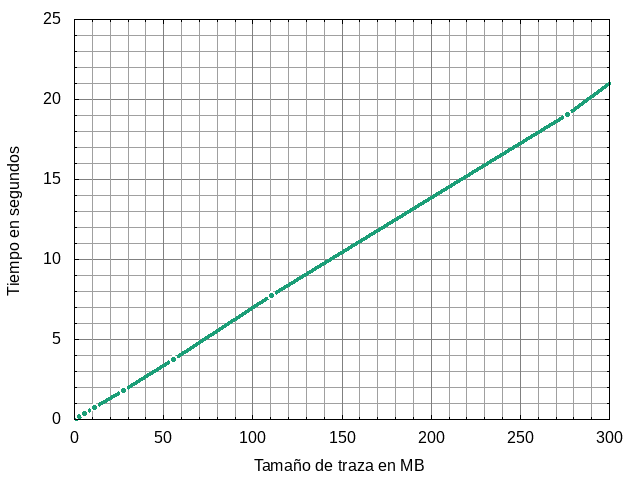
\includegraphics[scale=0.8]{latex/gnuplot/png/time.png}
\caption[Gráfica de tiempo de ejecución]{Tiempo de ejecución en función del tamaño de traza.}
\label{fig:Pruebas:Tiempo}
\end{figure}

Como se puede ver en la figura \ref{fig:Pruebas:Tiempo}, la relación entre el tiempo y el tamaño de la traza es claramente lineal. Se considera que el tiempo de procesado de los paquetes es rápido. Los 500 MB de memoria se corresponden a unos 10.000.000 de paquetes. Esta cantidad de paquetes puede entenderse como un rango de xxxxx tiempo en una empresa real. %TODO: ver a que cantidad de tiempo se corresponde para terminar el analisis

% TODO (Guillermo): Lo mismo aquí

\begin{figure}[H]
\centering
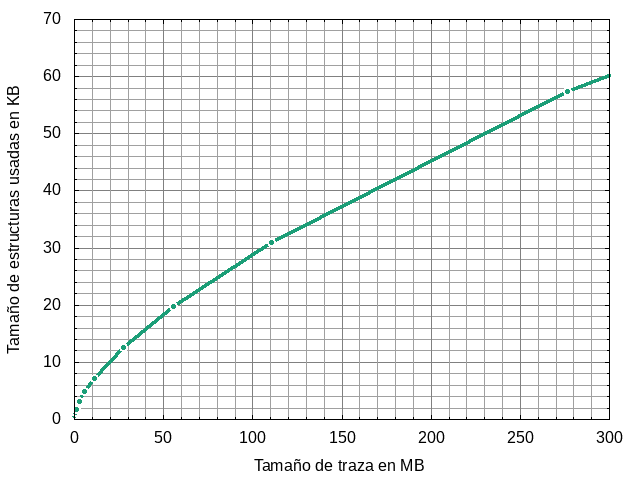
\includegraphics[scale=0.8]{latex/gnuplot/png/memory-usage.png}
\caption[Gráfica de memoria usada]{Memoria utilizada para la reserva de las estructuras en función del tamaño de traza.}
\label{fig:Pruebas:Memoria}
\end{figure}

En la figura \ref{fig:Pruebas:Memoria} podemos ver que el programa desarrollado es muy eficiente en memoria. Su eficiencia es mejor que $o(\sqrt{n})$ y, en general, la memoria usada en las estructuras durante el análisis es en promedio del 17\%, llegando a ser de solo el 0.9\% cuando se analizan 500 MB de traza. Se considera que la eficiencia en memoria es muy buena ya que se estarían usando cantidades de memoria muy inferiores a los tamaños de las trazas usadas. %TODO: Puede que haya que expresar estos datos de manera diferente e incluso hallar exactamente la relacion de eficiencia

\subsection{Estructuras reservadas}
En la sección \ref{subsec:Desarrollo:IPMAC:CoefPools} se desarrollo la idea de estimar la cantidad de estructuras que se iban a reservar de cada tipo para hacer el programa más eficiente en memoria. El cálculo del coeficiente $\alpha$ se puede hacer ahora experimentalmente gracias a las trazas reales en las que se ha usado el programa. Podemos comprobar ahora como evolucionan estas medidas en la figura \ref{fig:Pruebas:Estructuras}.

% TODO (Guillermo) Y aquí también hay que usar puntos.

\begin{figure}[H]
\centering
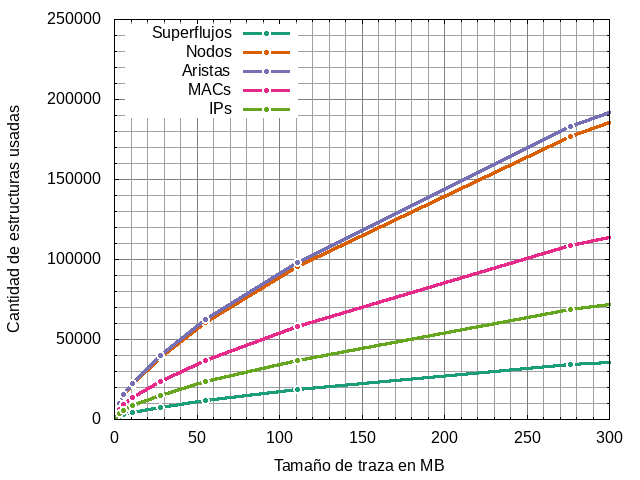
\includegraphics[scale=0.8]{latex/gnuplot/png/structures.png}
\caption[Gráfica de estructuras utilizadas]{Cantidad de estructuras reservadas en función del tamaño de traza.}
\label{fig:Pruebas:Estructuras}
\end{figure}

Se puede observar que los elementos que más estructuras acumulan son los nodos y las aristas. Esto es normal ya que el grafo de cada superflujo incluye varias de estas estructuras. Tras esto están las MACs y las IPs. Recordemos que en cada superflujo habrá únicamente dos IPs y que la relación de MACs por superflujo quedaba por estimar experimentalmente. Si tomamos todos los datos obtenidos y miramos los ratios de cada estructura por superflujo en promedio nos queda la tabla \ref{tab:Pruebas:Ratios estructuras}.

\begin{table}[hbtp]
	\centering
	\begin{tabular}{lccc}
		\toprule & \textbf{Ratio Teórico}  & \textbf{Ratio Teórico Estimado} & \textbf{Ratio Real} \\ 
		\midrule
		Superflujos & 1 & 1 & 1 \\
		Nodos & $2+\alpha$ & 4,94 & 4,94 \\
		Aristas & $(n-1)+\lambda$ & 3,94 & 4,87 \\
		MACs & $\alpha$ & 2,94 & 2,94 \\
		IPs & 2 & 2 & 2 \\ 
		\bottomrule
	\end{tabular}
	\caption{Ratios teóricos y experimentales de estructuras}
	\label{tab:Pruebas:Ratios estructuras}
\end{table}

Sustituimos los parámetros $\alpha = 0.0078$ (como se vio en \ref{sec:Analisis:Edges per node}) y $\alpha = 2,94$ (tomado del ratio real observado en la traza). Podemos ver que, aplicando las fórmulas de ratio teóricas la única diferencia se presenta en las aristas, donde las estimadas son menos que las reales. Esto se puede deber a que la primera aproximación que realizamos no fuera lo suficientemente exacta o a que, como ya se mencionó, las bifurcaciones que puede haber en cada red son muy diferentes y dependen de las características específicas de cada una. A nivel práctico, la conclusión que sacamos es que el parámetro $\lambda$ debe ajustarse para soportar redes con una gran cantidad de bifurcaciones. De esta manera, la pérdida de eficiencia en memoria será mínima en las redes con pocas bifurcaciones y el programa seguirá funcionando en redes con muchas bifurcaciones.

\chapter{Conclusiones}
\label{chap:Conclusiones}

\section{Conclusiones generales del proyecto}

\section{Trabajo futuro}

\backmatter
\appendix

\cleardoublepage

\nocite{*}
\bibliography{superflows}{}

\cleardoublepage
\printindex

\end{document}
